%%%\documentclass[option]{webofc}
%%% "twocolumn" for typesetting an article in two columns format (default one column)
%
\documentclass{webofc}
\usepackage[varg]{txfonts}   % Web of Conferences font
\usepackage[caption = false]{subfig}
\usepackage{float}
\usepackage{indentfirst}
\usepackage{inputenc}

%
\begin{document}
%
\title{Validation of a thermal non-equilibrium Eulerian-Eulerian multiphase
model of a 620 MWe pulverized fuel power boiler.}

\author{\firstname{Brad} \lastname{Rawlins}\inst{1}\fnsep\thanks{\email{rwlbra001@myuct.ac.za}} \and
        \firstname{Ryno} \lastname{Laubscher}\inst{1}\fnsep\thanks{\email{ryno.laubscher@uct.ac.za}} \and
        \firstname{Pieter} \lastname{Rousseau}\inst{1}\fnsep\thanks{\email{pieter.rousseau@uct.ac.za}}
        }

\institute{University of Cape Town, Department of Mechanical Engineering 
          }

\abstract{%
The use of a thermal non-equilibrium Eulerian-Eulerian model for the simulation of a 620 MWe power boiler is proposed for capturing the combustion and radiative heat transfer found in the pulverized fuel systems. The models eliminates the use of a Lagrangian reference frame in tracking solid fuel particles thereby reducing the computational expense and time. The model solves the scalar transport for the particle mass, energy and radiation interactions between the pseudo-particle and continuous phases. The goal is to apply the modelling approach to generate a simulation database for different load cases and firing conditions which in turn will be used to study flexible operation. The model is validated against both numerical and applicable site data measurements. It is shown that the model is able to adequately resolve the furnace and superheater wall heat fluxes. Additionally the resolution of the flow field, combustion dynamics and wall fluxes are demonstrated for both an 80\% and 60\% operational loads. Moreover, it is shown that the Eulerian-Eulerian model results in approximately a 30\% computational resource reduction when compared to traditional modelling approaches.
}
%
\maketitle
%
\section{Introduction}\label{intro}

The mid-merit operation of Coal-Fired Power Plants (CFPP) arises from the intermittent supply of electricity produced by renewable sources. Research into the flexible/mid-merit operation of power plants is needed to better understand the dynamic operations arising from these off-design conditions if renewable energy sources are to be integrated onto electrical grids.\\

Three-dimensional computational fluid dynamics (CFD) can capture the thermal performance of CFPPs at different load conditions with the necessary accuracy. These 3D CFD models include the modelling of combustion, radiation, and fluid flow phenomena. The traditional method for modelling
solid-fuel combustion systems, such as CFPPs, is acknowledged as the Eulerian-Lagrangian (EL) approach. Successful implementations, using the EL approach include the following studies \cite{bohnstein},\cite{laubscher_1} and \cite{laubscher_2}, where the latter focused on the effect that the burner swirl direction has on the heat uptake to the furnace and superheater walls of a 620 MWe boiler.\\

Another approach is to use a Eulerian multi-fluid model as used by the following studies \cite{epple}, \cite{cai} and \cite{wu}. Knaus et al \cite{knaus} compared the Eulerian-Eulerian (EE) and EL approaches for a 550 MWe coal-fired utility boiler. The predicted combustion products yield only small differences, with carbon monoxide being better predicted when using the Eulerian-Lagrangian approach. The computational effort of the Eulerian approach proved more efficient and faster convergence times were noted. It should be stated, that these studies were conducted using in-house CFD codes which is difficult to apply by engineers and scientists outside the research group.\\

The current work proposes the use of an EE modelling strategy that incorporates thermal non-equilibrium between the gas and particle phases which allows for adequate particle concentration tracking and heat transfer interactions, with a reduced computational cost when compared to the EL simulation approach. The model is validated for a full scale utility power boiler for various load cases. The validated modelling technique is to be used for future studies in developing a CFD data-driven surrogate model of a 620 MWe CFPP's furnace and radiant superheaters. 

\section{Mathematical model} \label{Theory}
\subsection{Numerical modelling methodology}
An outline of the modelling methodology, utilized by the proposed EE model, is provided in this section highlighting the general conservation equations, pseudo-solid phase tracking, and the combustion and radiation modelling techniques employed. The basis of the model assumes that the gas and solid phases behave as inter penetrating continua with both phases being described in a Eulerian reference frame. A further assumption is that the fluid is in dynamical equilibrium with the solid phase, (similar to the work of \cite{epple}), meaning that velocities of both phases are locally the same.

\subsubsection{Transport equations}
The time-averaged steady-state continuity, momentum, k-$\epsilon$ turbulence  and energy equations for the gas-phase can all expressed using the following generalised transport equation for a variable $\phi$ expressed as:

\begin{equation}\label{eqn_general}
\underbrace{\frac{\partial}{\partial x_{i}}(\rho u_{i}\phi)}_{\text{Advection}}= \underbrace{\frac{\partial}{\partial x_{i}}(\Gamma_{\phi}\frac{\partial \phi}{\partial x_{i}})}_{\text{Diffusion}}+\underbrace{S_{\phi}}_{\text{Source}} 
\end{equation}
where $\rho$ is the gas density and $\Gamma_{\phi}$ is the diffusion coefficient for variable $\phi$.\\

In the present work the flue gas phase is modelled using the species-transport approach where a transport equation is solved for each constituent mass fraction in the gas mixture. The governing equations for the gas phase can be written as follows;\\

Mass conservation:
\begin{equation}\label{eqn_RANS_mass}
\frac{\partial}{\partial x_{i}}(\rho \bar{u}_{i})=S_{m}.
\end{equation}
Momentum conservation:
\\
\begin{equation}\label{eqn_momentum}
\frac{\partial}{\partial x_{i}}(\rho_{eff} u_{i}u_{j})+\frac{\partial \overline{P}}{\partial x_{j}}=\frac{\partial}{\partial x_{i}}\left[\mu\left\{\frac{\partial u_{j}}{\partial x_{i}}+\frac{\partial u_{i}}{\partial x_{j}}-\frac{2}{3}\delta_{ij}\frac{\partial u_{i}}{\partial x_{i}}\right\}\right]+\frac{\partial}{\partial x_{i}}(-\rho\overline{u_{i}^{'}u_{j}^{'}})+S_m
\end{equation}\\

The momentum equation is closed by approximating the Reynolds stresses using the Boussinesq relationship as shown in equation \eqref{eqn_bouss}.
\begin{equation}\label{eqn_bouss}
-\rho\overline{u_{i}^{'}u_{j}^{'}}=\mu_{t}\left(\frac{\partial u_{i}}{\partial x_{j}}+\frac{\partial u_{j}}{\partial x_{i}}\right)-\frac{2}{3}\left(\rho k+\mu_{t}\delta_{ij}\frac{\partial u_{k}}{\partial x_{k}}\right)
\end{equation}

This approximation is used in conjunction with the realizable k-$\epsilon$ turbulence model of Shih et al \cite{shih}\\

Energy conservation:
\begin{equation}\label{eqn_energy}
\frac{\partial }{\partial x_{i}} (u_{i}[\rho E+P])=\frac{\partial }{\partial x_{j}}\left[\lambda\frac{\partial T_{g}}{\partial x_{j}}\right] +S_{h}
\end{equation}
where $E$ in the total energy term, $P$ the pressure, $\lambda$ is the effective thermal conductivity and $T_g$ is the gas temperature.\\

Species transport:
\begin{equation}\label{eqn_species}
\begin{split}
&\frac{\partial}{\partial x_{i}}(\rho u_{j}Y_{k})=-\frac{\partial}{\partial x_{j}}(\vec{J_{k}})+ \sum_r R_{j,r} + S_{k}\\
&k = 1,2,3...N
\end{split}
\end{equation}
where $k$ is the number of species present in the domain and $\vec{J_{k}}$ is the species diffusion flux. $\sum_r R_{j,k}$ is the net rate of production of species $j$ due to $r$ reactions.\\

To correctly account for the particle inertial effects on the gas phase convection an effective density is defined as follows and is used in the above equations.

\begin{equation} \label{eff_rho}
	\rho_{eff} = \frac{\rho \rho_p \left( \phi_{mp} + 1 \right)}{\rho \phi_{mp} + \rho_p}
\end{equation}

In equation \eqref{eff_rho}, $\rho_p$ is the particulate matter density and $\phi_{mp}$ $[kg_p/kg]$ is the local mass concentration of particulate matter present in the gas volume. 
\\
\subsubsection{Solid phase modelling}
The pseudo particles transported into the domain are modelled using a scalar field and transported through the computational domain according to equation \eqref{eqn_general}. The pseudo particle scalar fields are used to define the fuel characteristics based on the proximate analysis composition (refer to Table \ref{tab_fuel}), namely consisting of moisture, volatile matter, fixed  carbon and ash. Each of the scalar field equations solved for are given in Table \ref{tab_scalars}.\\

\begin{table}[h!]
\centering
\caption{Scalar field equation descriptions}\label{tab_scalars}       
\begin{tabular}{lll}
\hline
Variable &Description& Transport equation \\
\hline
$\phi_{mp0}$ &Original/initial mass of particles& $\frac{\partial}{\partial x_{i}}(\rho u_{i} \phi_{mp0})=0$\\
$\phi_{M}$&Moisture present in particles&$\frac{\partial}{\partial x_{i}}(\rho u_{i} \phi_{M})=\frac{1}{V} \frac{dM_{evap}}{dt}$\\
$\phi_{VM}$&Volatile matter present in particles&  $\frac{\partial}{\partial x_{i}}(\rho u_{i} \phi_{VM})=\frac{1}{V}\frac{dM_{devol}}{dt}$\\
$\phi_{FC}$&Fixed carbon present in particles&$\frac{\partial}{\partial x_{i}}(\rho u_{i} \phi_{FC})=\frac{1}{V}\frac{dM_c}{dt}$\\
$\phi_{ASH}$&Ash present in particles&$\frac{\partial}{\partial x_{i}}(\rho u_{i} \phi_{ASH})=0$\\
$\phi_{hp}$&Enthalpy of particle&Equation \eqref{eqn_phi_hp}\\
\hline
\end{tabular}
\end{table}

The energy transport of the pseudo particle, is transported by defining the particle enthalpy using the following equation:
\begin{equation}\label{eqn_phi_hp}
\frac{\partial}{\partial x_{i}}(\rho u_{i} \phi_{hp})=\left(f_{heat}\frac{dM_{c}}{dt}h_{rxn} + \dot{Q}_{rad} + \dot{Q}_{conv} - \frac{dM_{evap}}{dt}h_{fg}\right)\frac{1}{V}
\end{equation}

The equation accounts for all the processes associated with energy transport to the particle, namely convection $\left(\dot{Q}_{conv}\right)$, radiation $\left(\dot{Q}_{rad}\right)$, latent heat $\left(\frac{dM_{evap}}{dt}h_{fg}\right)$ and near surface char oxidation $\left(f_{heat}\frac{dM_{c}}{dt}h_{rxn}\right)$. This gives the model the ability to track the particle temperature in the domain, moving the model away from the thermal equilibrium approach incorporated by previous studies using an EE approach (\cite{epple}, \cite{knaus}). The particle temperature is important in describing the sequential steps found in modelling combustion processes, especially at low boiler loads where mixing and ignition become problematic.

\subsubsection{Combustion modelling}
The combustion modelling of coal comprises four sequential steps, namely the heating/cooling of the particles, evaporation, devolatilization and char oxidation. The process starts with the pseudo-particles entering the domain and heating up until the moisture's boiling temperature of 373 K is reached \cite{cengel}. The realization of the boiling temperature would release moisture based on a boiling rate which is defined as:

\begin{equation}\label{eqn_evap_release}
\frac{dM_{evap}}{dt}h_{fg}=\dot{Q}_{rad} + \dot{Q}_{conv}.
\end{equation}

Following this is the devolatilization process whereby the volatiles present in the fuel are liberated. The initialization temperature of the devolatilization process was found to vary between $553 - 623\;K$ for a variety of coals by Ranade and Gupta \cite{gupta}, thus particle heating would need to ensue after the moisture evaporation to bring the particles to the initialization temperature. A single-step Arrhenius kinetic rate model is used to approximate the devolatilization process since these models can predict the devolatilization of coal and are simpler to implement, according to Sankar et al \cite{sankar}). The rate is expressed in equation \eqref{eqn_vol_release} as:\\
\begin{equation}\label{eqn_vol_release}
\frac{dM_{vol}}{dt}=R_{vol}(m_{0,vol}-m_{vol}).
\end{equation}
where $R_{vol} = A_{vol} \exp(-E_{a,vol} / R T_p)$, with $A_{vol} = 2E5$ $[s^{-1}]$ and $E_{a,vol} = 6.7E7$ $[J/kmol]$  from the works of Sheng et al \cite{sheng}. Here $m_{vol}$ is the mass of the volatile released during combustion and $m_{0,vol}$ is the initial volatile mass present before combustion.\\

The final step of the solid fuel combustion process is realized when all the volatiles have been driven off from the pseudo-particles. The product species of the char oxidation process is CO, with 100\% of the resultant heat being absorbed by the pseudo-particle contributing to the energy rise of the particle matter in a cell. The char oxidation rate is derived from the works of Baum and Street \cite{baum} and Spalding \cite{spalding}. The model is commonly referred to as the diffusion-kinetics limited model, written as:
\begin{equation}\label{eqn_char_release}
\frac{dM_c}{dt}=-A_{p}\frac{R_{c}R_{diff}}{R_{c}+R_{diff}}P_{O_{2}}
\end{equation}

The interested reader is directed to \cite{ansys} for an in-depth derivation of the above equation. The kinetic parameter $R_{c} = A_{c} \exp(-E_{a,c} / R T_p)$, where $A_c = 0.0053$ $[kg/m^3]$ and $E_{a,c} = 8.37E7$ $[J/kmol]$ from the works of Sheng et al \cite{sheng} and Hanjalić et al \cite{han}. Here $A_p$ is the particle surface area, $R_{diff} = (5E-12)(0.5(T_p+T_g))^{0.75})/\bar{d_p}$ is the diffusion rate coefficient, which is a function of the gas and pseudo-particle temperature and average diameter,  and $P_{O_{2}}$ is the partial pressure of oxygen.\\

According to Sankar et al \cite{sankar}, the gas phase reactions in boilers are fast, with the chemical time scales being orders of magnitude faster than turbulent mixing time scales. This leads to a mixed-is burnt assumption \cite{dibble}, which assumes the chemistry is infinitely fast and irreversible, being adequate for species and temperature distribution predictions. The gas-phase volatile and CO reactions are approximated using the two-step global reaction shown in equation \eqref{eqn_volatiles}. 
\begin{equation}\label{eqn_volatiles}
\begin{split}
&\underbrace{CH_{3.51}O_{0.78}N_{0.1106}S_{0.0466}}_{Volatiles}+1.03O_2\to CO + 1.75H_2O + 0.0466SO_{2} + 0.0553N_2\\
&CO + 0.5O_2\to CO_2
\end{split}
\end{equation}

This study makes use of the two-step finite-rate/eddy-dissipation model (FR/EDM) in ANSYS Fluent® 19.3 \cite{ansys} to calculate the gaseous reaction rates. The model calculates three rates and uses the minimum of the three values for the source term calculations for the species transport equations and subsequently for the energy release source terms.
Chemical reaction rate:
\begin{equation}\label{eqn_rate_chemical}
R_{j,r,chemical}=A_{r}exp\left(\frac{-E_{a,r}}{RT_g}\right)\left[\vartheta^{'}_{k,r}-\vartheta_{k,r}\right]\prod_{L}\left[C_{l,r}\right]^{m,r}
\end{equation}
Rate of turbulent production eddies dissipation:
\begin{equation}\label{eqn_rate_products}
R_{j,r,prodcution}=\vartheta_{k,r}M_{w,k}AB\rho\frac{\varepsilon}{k}min\left(\frac{\sum_{p} Y_p}{\sum_{j}\vartheta_{j,r}M_{w,j}}\right)
\end{equation}
Rate of reaction eddies dissipation:
\begin{equation}\label{eqn_rate_reactants}
R_{j,r,reactant}=\vartheta_{k,r}M_{w,k}A\rho\frac{\varepsilon}{k}min\left(\frac{Y_R}{\varepsilon_{R,r}M_{w,R}}\right)
\end{equation}

In the above equations $Y_p$ is the product species mass fraction, $Y_R$ is the mass fraction of any reaction species, $A$ and $B$ are model constants, $M_{w,k}$ is the molecular weight of $j^{th}$ species, $\vartheta_{k,r}$ is the stoichiometric coefficient of reactant $k$ in reaction $r$, $[C_{l,r}]^{m,r}$ is the molar concentration of species $l$ in reaction $r$ with rate exponent $m$, $A_r=2.56E11$ $[s^{-1}]$ and $E_{a,r}=1.081E8$ $[J/kmol]$ taken from the study of He et al \cite{he}.   
\subsubsection{Radiation modelling}

The heat transfer to the furnace, platen and final superheater walls of the validation case are mainly due to radiation. The radiation transport for the current work was resolved using the P1 radiation model which includes the effects of particle absorption ($\alpha_p$) and scattering ($\sigma_p$) as well as gas mixture absorption ($\alpha_g$). The P1 model transport variable is the incident radiation (G - $W/m^2$), and can be written for a particle laden domain as:
\begin{equation}
\begin{split}
&\frac{\partial}{\partial x_{i}}\left(\Gamma\frac{\partial G}{\partial x_{i}}\right)=\left(\alpha_g+\alpha_p\right)G-4\left(\alpha_g \sigma_{SB} T_{g}^4-\pi E_p \right)\\
&\Gamma = \frac{1}{\alpha_g+\alpha_p+\sigma_p}
\end{split}
\end{equation}

The gas mixture absorption coefficient was calculated using the weighted sum of gray gases model (WSGGM) which accounts for the tri-atomic gases $CO_2$ and $H_2O$ as proposed by Smith et al \cite{smith}. The solid phase radiative properties (namely $\alpha_p$, $\sigma_p$ and $E_p$) were determined using an equivalent Eulerian description for each expressed as:\\
\begin{equation}
\alpha_p \equiv \frac{\epsilon_{p,n}A_{proj}N_p}{V}
\end{equation}
\begin{equation}
\sigma_p \equiv (1-\epsilon_{p,n})(1-f_p)\frac{A_{proj} N_p}{V}
\end{equation} 
\begin{equation}
E_p \equiv \frac{\epsilon_{p,n}A_{proj}\sigma_{SB} T_{p}^4 N_p}{\pi V}
\end{equation}
where $N_p = \rho \phi_{mp0} V / \left( \rho_p \pi \bar{d_p}^3 /6 \right)$, is the number of particles present based on the average diameter pseudo particle size $\bar{d_p}$, $A_{proj} = N_p \pi d_p^2 / 4 V$ is the projected area, $\sigma_{SB} = 5.67E-8 ;[W/m^2K^4]$, $T_p$ is the particle temperature and $V$ is the cell volume. The particles emissivity ($\epsilon_p$) and scattering factor ($f_p$) were implemented using a variable property correlation as used in the work of Laubscher and Rousseau \cite{laubscher_3}.
\newpage

\subsection{Numerical setup and model inputs} \label{Setup}
The modelling methodology, described previously, was successfully incorporated in the modelling of a 620 MWe subcritical power boiler. Figure \ref{comp_dom} illustrates the computational domain used in this validation study highlighting the various heat receiving surfaces and inlets. The burner feeds the combustion chamber with primary and secondary air through the burners inner and outer annuli respectively. At 100\% maximum continuous rating (MCR) the primary air (PA) supplies the fuel and air at a temperature of 373 K and secondary air (SA) enters at a temperature of 577 K.\\
\begin{figure}[h!]
\centering
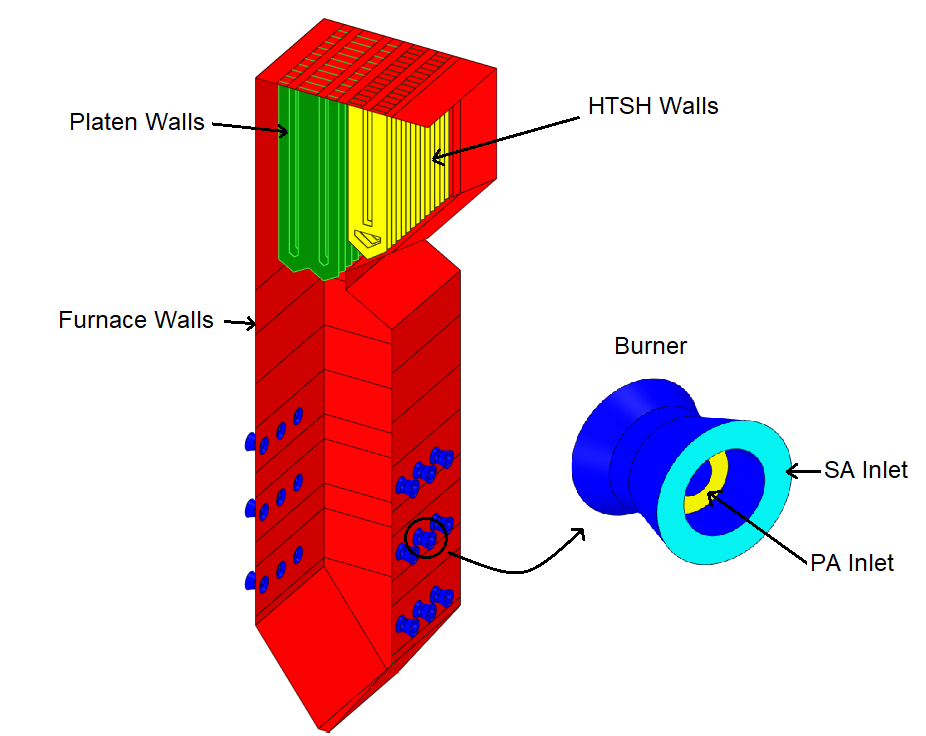
\includegraphics[scale=0.375]{domain}
\setlength{\belowcaptionskip}{0pt}
\caption{Computational domain layout}
\label{comp_dom}
\end{figure} \\
The fuel characteristics used for CFD modelling purposes are given in Table \ref{tab_fuel}.
\begin{table}[h!]
\centering
\caption{Fuel characteristics used in CFD model} \label{tab_fuel}
\begin{tabular}{ll}
\hline
Fuel constituent & Fraction - ($kg/kg_{fuel}$)   \\
\hline
\textit{Ultimate analysis - [Dry-Ash-Free]} & -  \\
C & 0.775 \\
H & 0.042 \\
N & 0.018 \\
O & 0.147 \\
S & 0.018 \\
\textit{Proximate analysis - [As-received]} & -\\
Fixed Carbon & 0.34\\
Volatiles & 0.196\\
Ash & 0.409\\
H\textsubscript{2}O & 0.055\\
\hline
Energy Content & As-received - ($kJ/kg_{fuel}$)\\
\hline
Higher Heating Value - (HHV) & 15070 \\
\hline
\end{tabular}
\end{table}

The plant in designed to operate at a 100\% MCR with a excess air ratio of 15.5\%. As the plant is turned down from 100\% MCR the excess air ratio is increased to ensure sufficient air and fuel mixing occurs. At MCR ratings of 81\% and 60\% the excess ratios were calculated as 20.9\% and 26.3\% respectively, based on the design schedule data. The inlet mass flow rates and temperatures for the plant's MCR ratings of 100\%, 81\% and 60\% are listed in Table \ref{tab_inlets}.
\begin{table}[h!]
\centering
\caption{Inlet conditions for simulated load cases (per burner)}\label{tab_inlets}       
\begin{tabular}{llllc}
\hline
Load Rating & 100 \% & 80 \% & 60 \% & Unit  \\
\hline
PA flow rate & 4.75 & 4.01 & 2.81 & $kg/s$   \\
SA flow rate & 14.27 & 12.04 & 8.43 & $kg/s$ \\
Fuel flow rate & 3.12 & 2.52 & 1.67 & $kg/s$ \\
PA inlet temperature & 373.15 & 373.15 & 373.15 & $K$ \\
SA inlet temperature & 577.15 &558.15 & 535.15 & $K$  \\
\hline
\end{tabular}
\end{table}\\
Other required wall boundary conditions such as wall temperatures and emissivities are listed in the work of Laubscher and Rousseau \cite{laubscher_1}.
\subsubsection{Numerical solution strategy}
The current simulations were performed using the ANSYS Fluent\textsuperscript{\textregistered} 19.2 pressure-based solver. Pressure-momentum coupling was set to the SIMPLE technique, with momentum, energy and species equations being discretized using the second-order upwind method. The pressure equation was discretized using PRESTO!. This setup holds for both the EE model and the detailed EL model. The difference arises in the use of scalar fields in the EE configuration and using the discrete phase modelling approach in the EL setup. Simulations were performed on a numerical mesh consisting of roughly 6.2 million cells. A mesh independence study was conducted for mesh sizes consisting of 4.2 and 10.2 millions with the 6.2 million cell model deemed acceptable for this study. To ensure an accurate numerical solution the mesh aspect ratio was kept below 15 and the minimum orthogonal quality above 0.2. The discrete phase equations, for the EL model, were solved once every 30 fluid phase iterations. The number of particles injected per burner was set to about 7800, totalling to 140 000 particles in the entire domain. To ensure a stable converged solution the spatial discretization for all fields were set to first order upwind (except pressure) and solved for 1500 iterations before increasing the discretization order. The simulations were then run for a further 10000 iterations. For all cases the maximum mass imbalance was 0.046 kg/s for a total gas flow rate of 376 kg/s. The maximum heat imbalance was 2450 kW for a total heat input of 855 MW.

\section{Results and discussion} \label{Results}

The discussion herewith compares the results of an EL numerical model with the results of the developed EE modelling approach, (discussed in section \ref{Theory}) for a 100\%, 81\% and 60\% MCR loads cases. Overall a 30\% (9 hours to approximately 6 hours) decrease in simulation time was observed across the simulated load cases.  \\ 

Table \ref{tab_rel_err} highlights the relative errors obtained between the EL and EE numerical models. A maximum error of 8.15\% occurs at the platen superheater for the 100\% load case. The relative errors are deemed acceptable for the decrease in computational time required by the EE model.
\begin{table}[h!]
\centering
\caption{Relative percentage errors of key parameters between the EL and EE models}\label{tab_rel_err}       
\begin{tabular}{llll}
\hline
Load Rating & 100\% & 80\% & 60\%   \\
\hline
Furnace heat load & 4.05\% & 8.15\% & 1.23\%   \\
Platen heat load & 6.93\% & 7.36\% & 7.21\%   \\
HTSH heat load & 2.81\% & 3.78\% & 4.23\%  \\
Furnace exit temperature & 3.56\% & 4.76\% & 5.62\%  \\
Exit X\textsubscript{CO\textsubscript{2}} fraction & 2.12\% & 1.56\% & 0.98\% \\
Exit X\textsubscript{O\textsubscript{2}} fraction & 1.86\% &3.21\% & 2.84\%\\
\hline
\end{tabular}
\end{table}

The graphs shown in figure \ref{fig_heat_load} illustrate the calculated (based off operational plant measurements), EL and EE models results,  for the heat loads to the furnace, platen and high temperature superheater (HTSH) walls.

\begin{figure}[h!]
\centering
\subfloat[100\% load case]{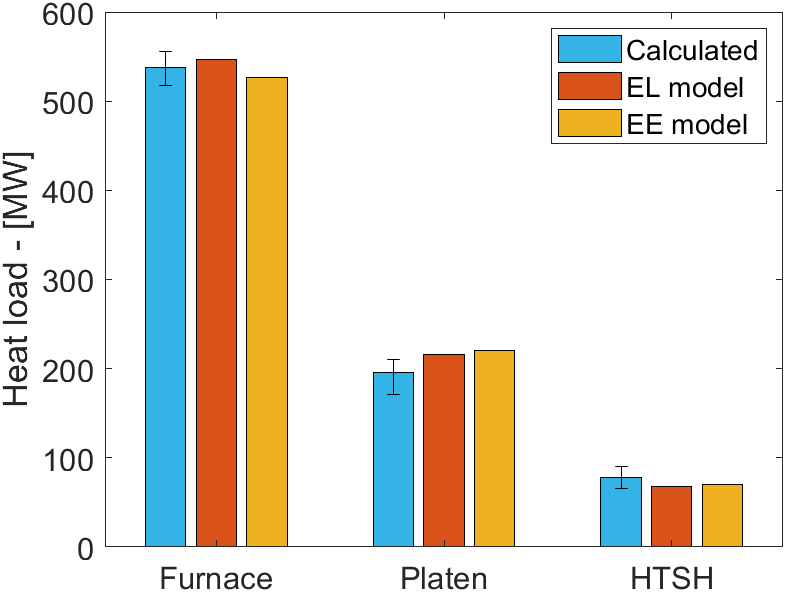
\includegraphics[width = 4cm, height = 3.2cm,  keepaspectratio]{bar_100}}
\hspace{2mm}
\subfloat[81\% load case]{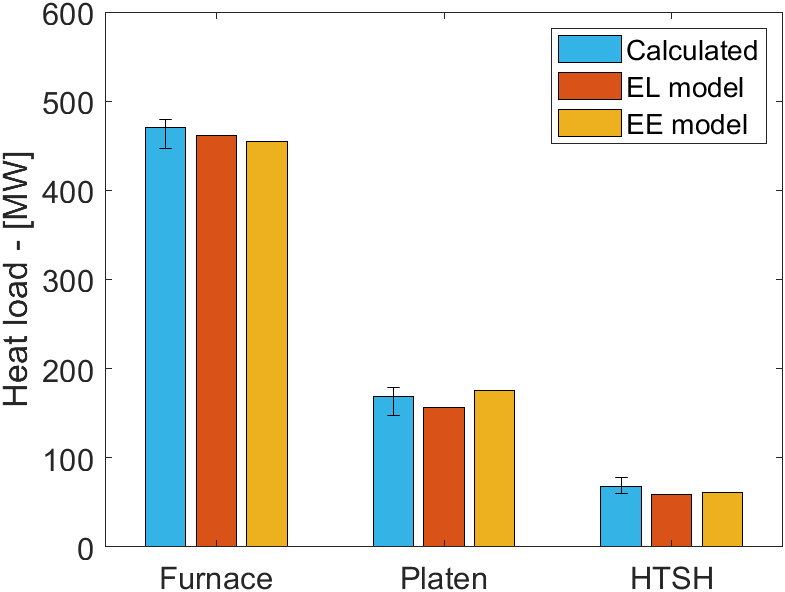
\includegraphics[width = 4cm, height = 3.2cm,  keepaspectratio]{bar_80}}
\hspace{2mm}
\subfloat[60\% load case]{\label{fig_heat_load_c}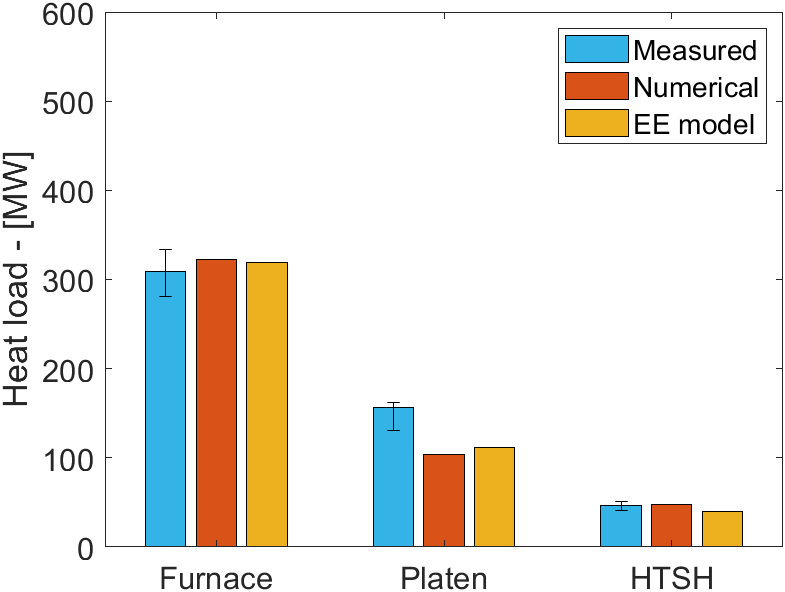
\includegraphics[width =4cm, height = 3.2cm,  keepaspectratio]{bar_60}} 
\setlength{\belowcaptionskip}{0pt}
\caption{Overall heat load performance for 100\%, 81\% and 60\% MCR load cases}
\label{fig_heat_load}
\end{figure}

The general accuracy of the EE model is seen to be able to sufficiently capture the overall heat loads when compared to the calculated and EL model results. A notable difference is seen in the 60\% load case of figure \ref{fig_heat_load} (c), where both the EL and EE numerical models under-predict the platens heat load. Figure \ref{fig_velocity} compares the gas velocity fields for the EL and EE model. It can be seen that results are in good agreement. The EE model tends to under predict the lower burner velocity transport resulting in combustion occurring closer to the burner mouth and lower furnace walls. This effect is seen in both the temperature contour plots of figure \ref{fig_temp} (d-f) and wall heat flux contours of figure \ref{fig_wall_heat} (d-f).
\begin{figure}[h!]
\centering
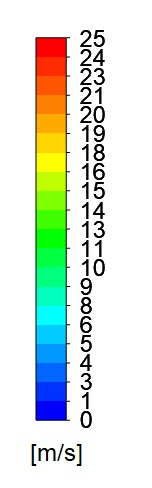
\includegraphics[scale = 0.3]{velo}
\subfloat[100\% case]{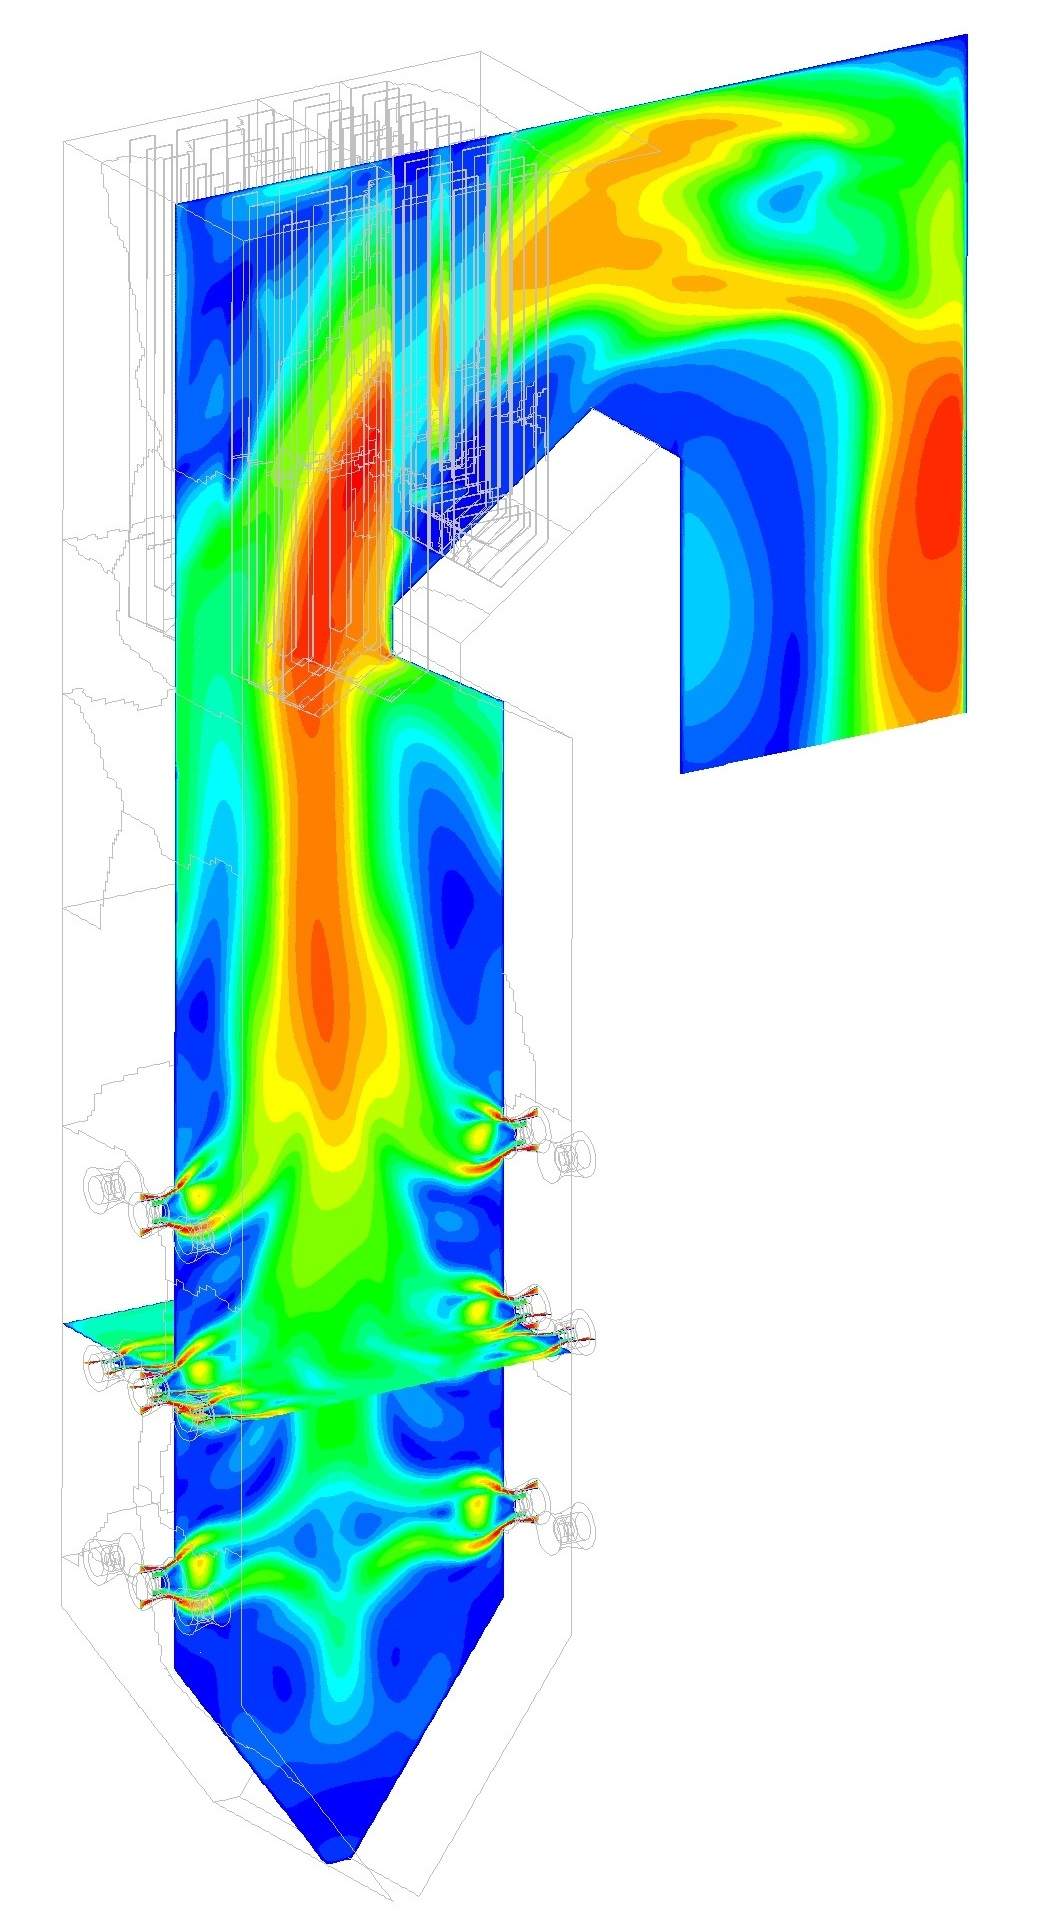
\includegraphics[scale = 0.0725]{100_velo}}
\hspace{10mm} 
\subfloat[81\% case]{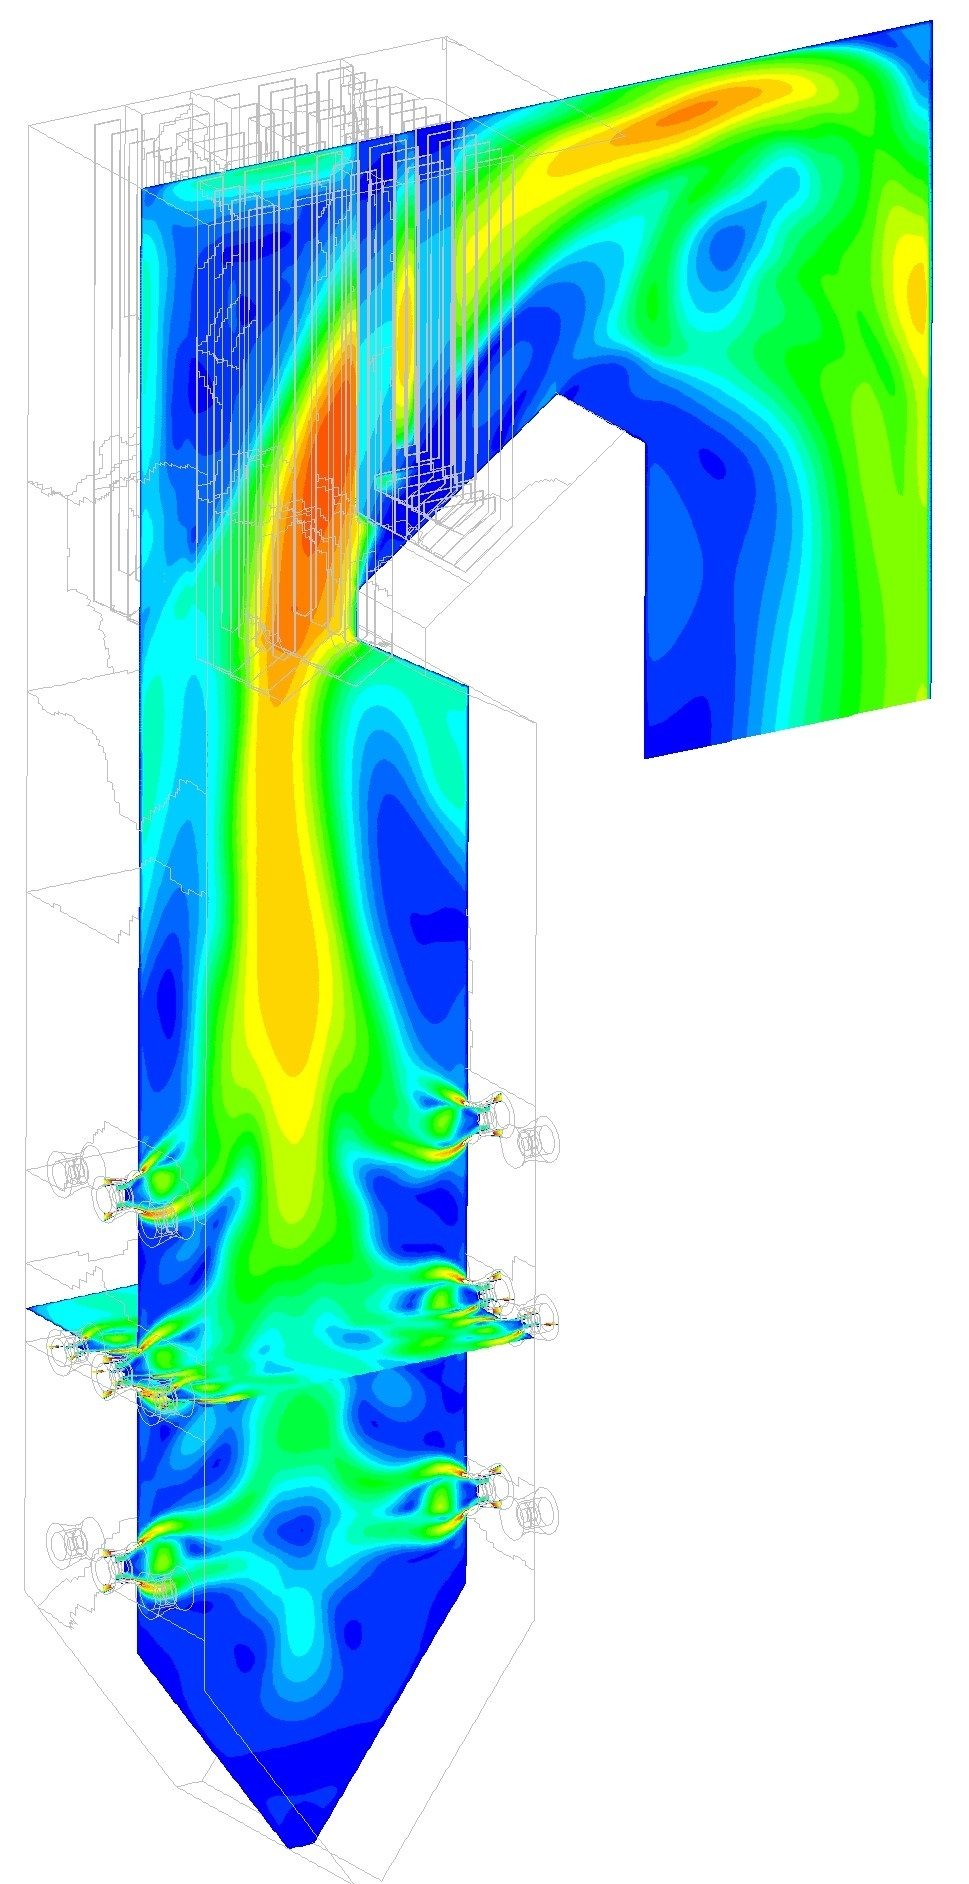
\includegraphics[scale = 0.0725]{80_velo}}
\hspace{10mm} 
\subfloat[60\% case]{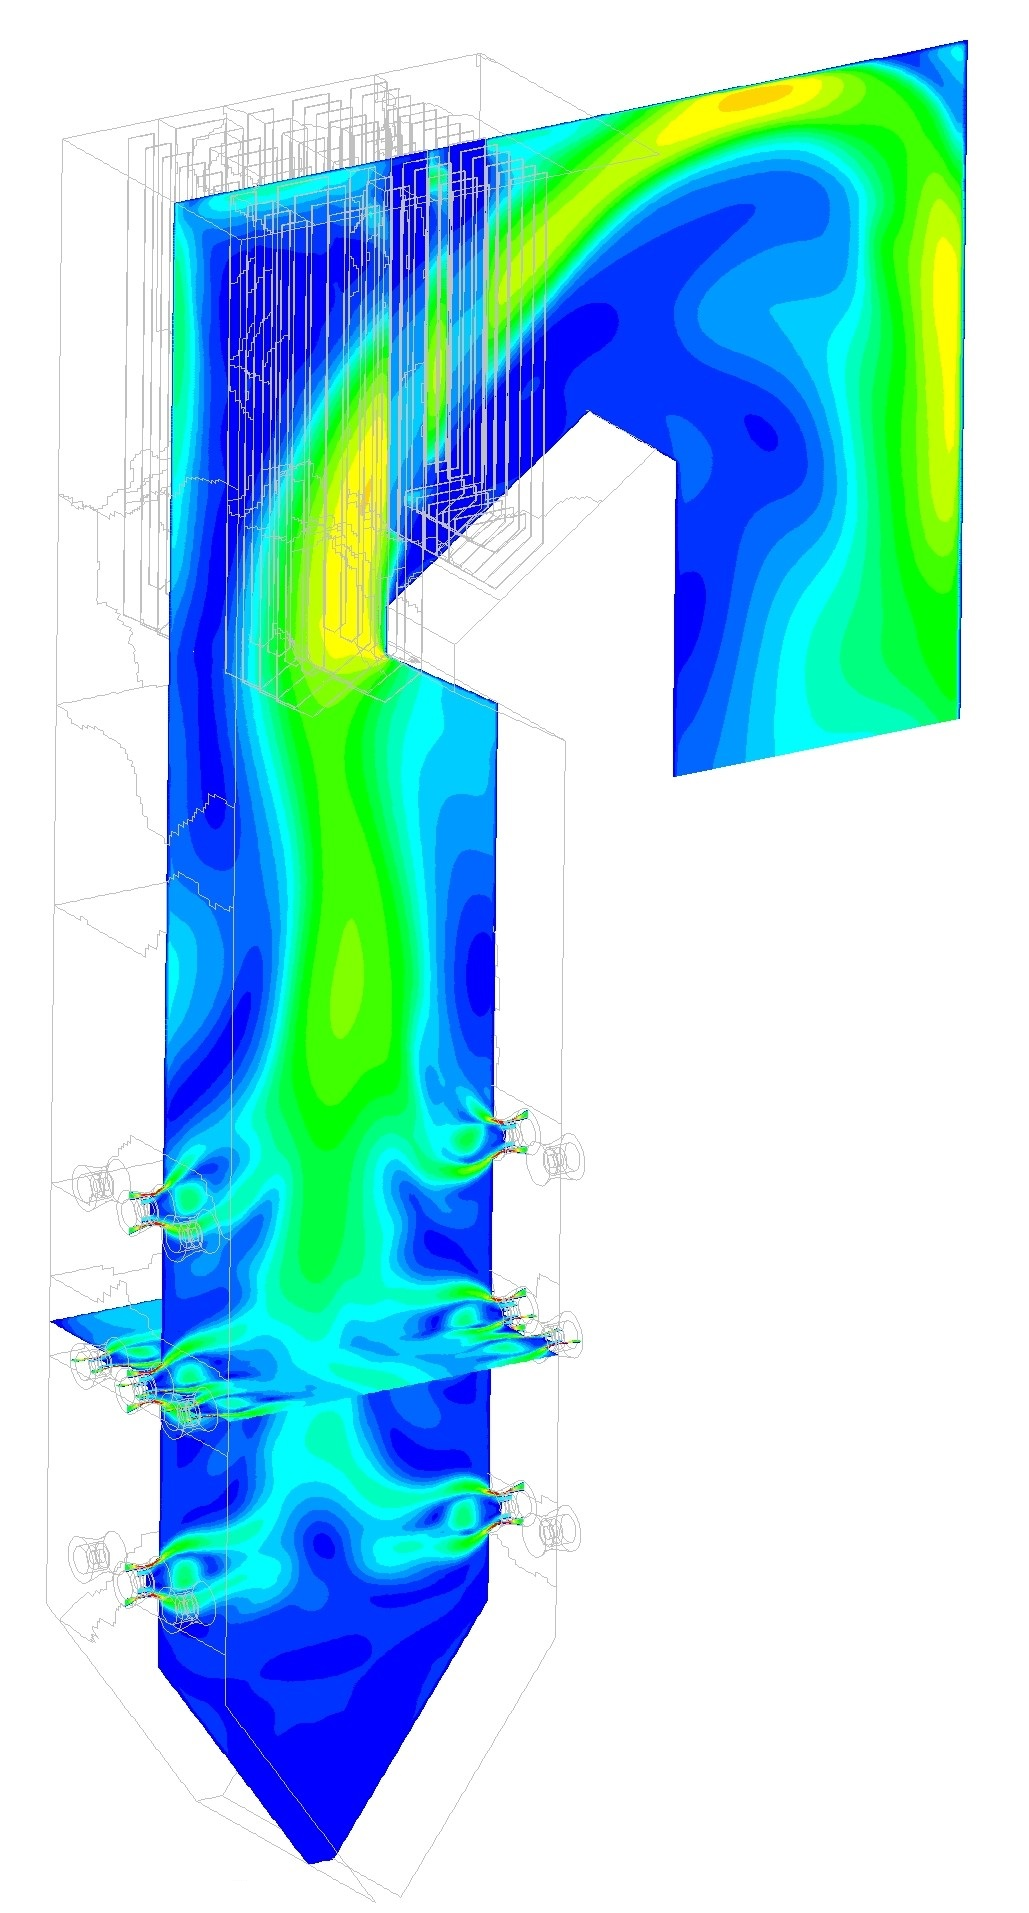
\includegraphics[scale = 0.0725]{60_velo}}\\
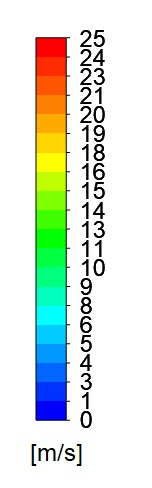
\includegraphics[scale = 0.3]{velo}
\subfloat[100\% case]{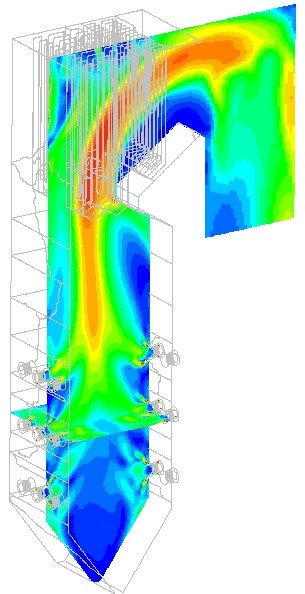
\includegraphics[scale = 0.224]{100_velo_spm}}
\hspace{10mm} 
\subfloat[81\% case]{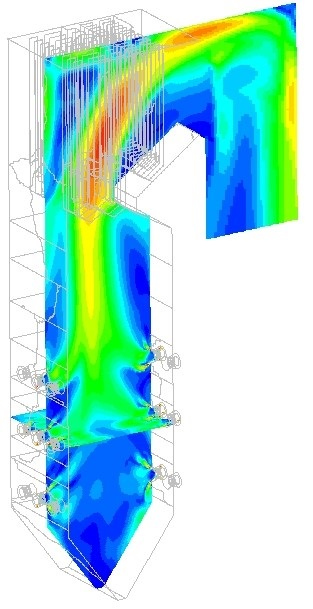
\includegraphics[scale = 0.224]{80_velo_spm}} 
\hspace{10mm} 
\subfloat[60\% case]{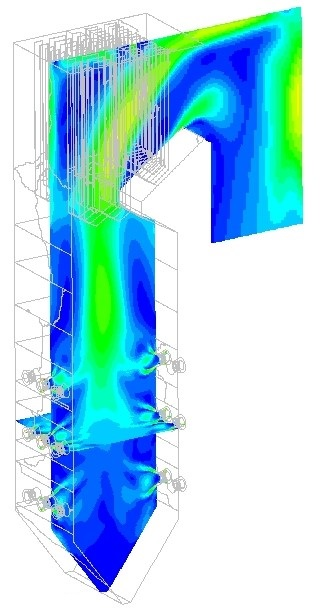
\includegraphics[scale = 0.224]{60_velo_spm}} 
\setlength{\belowcaptionskip}{0pt}
\caption{Gas velocity contour plots for the EL (a-c) and EE model (d-f) simulated load cases}
\label{fig_velocity}
\end{figure}
\\
\begin{figure}[h!]
\centering
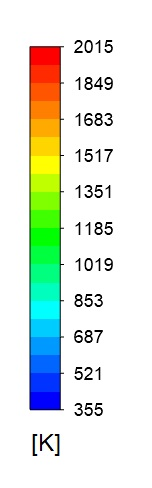
\includegraphics[scale = 0.3]{temp} 
\subfloat[100\% case]{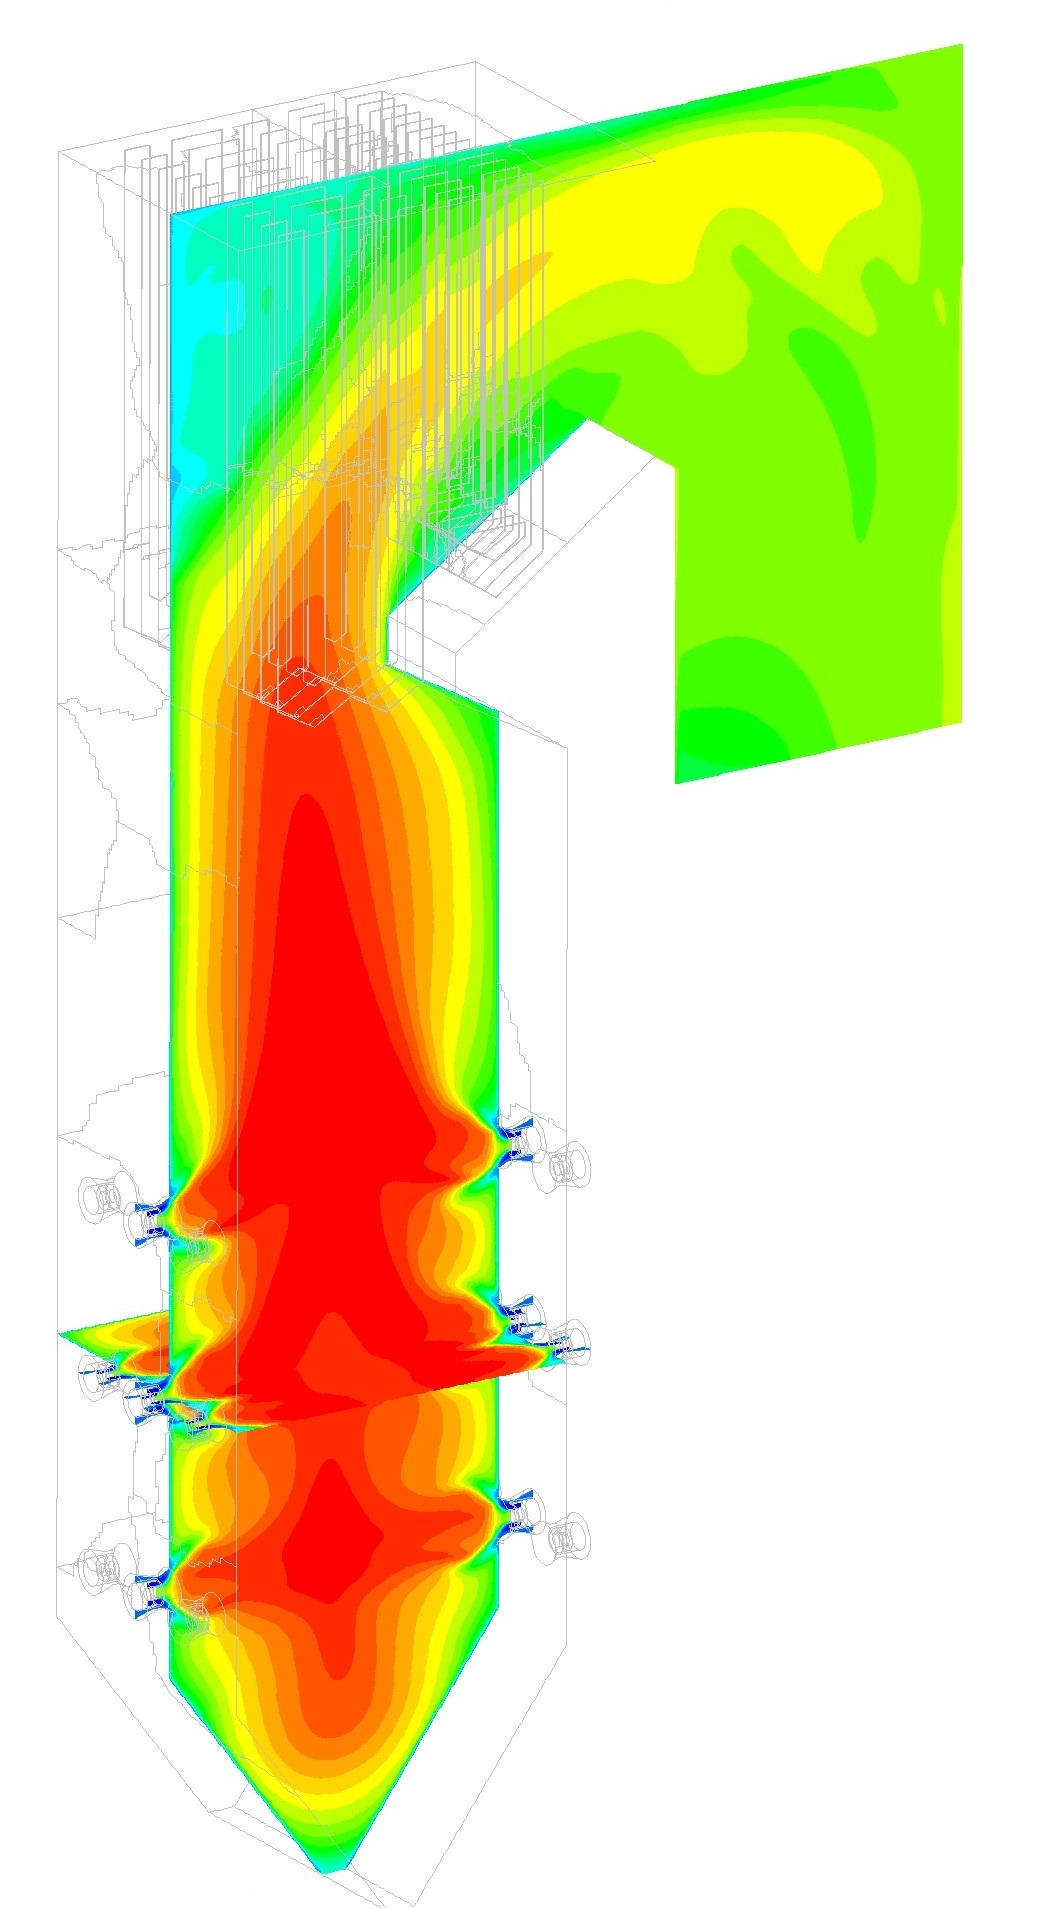
\includegraphics[scale = 0.0725]{100_temp}}
\hspace{10mm}  
\subfloat[81\% case]{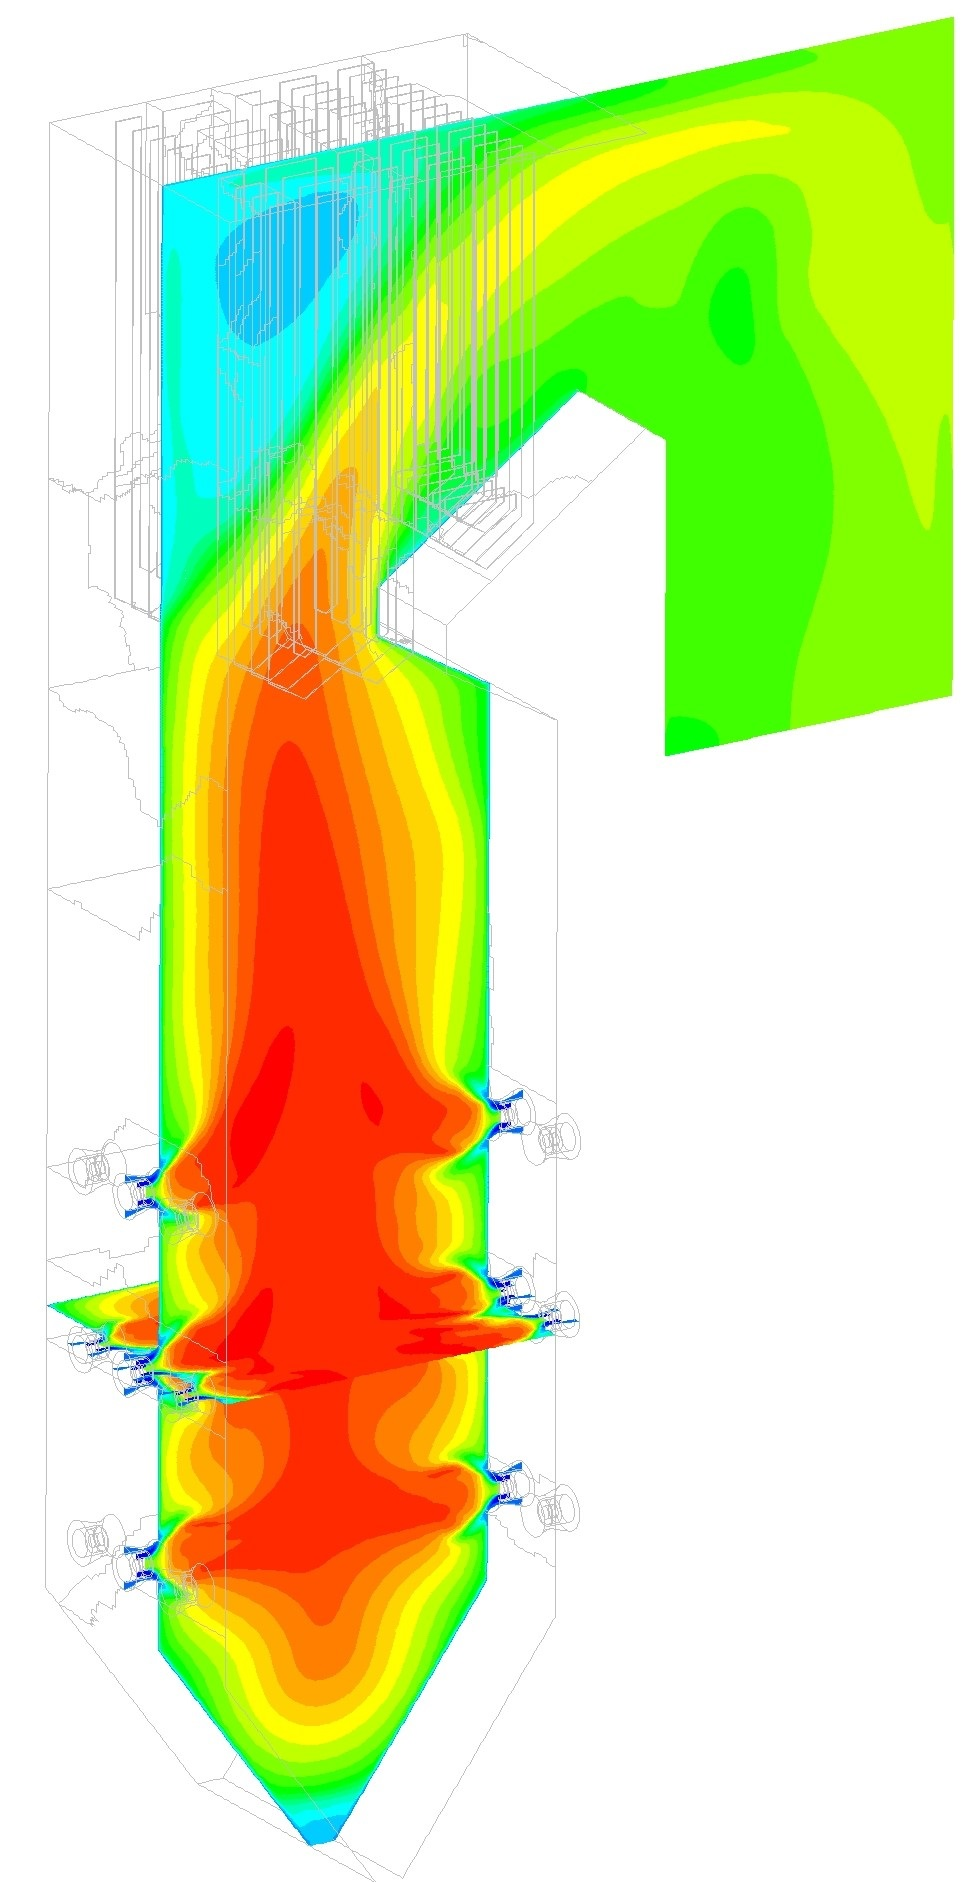
\includegraphics[scale = 0.0725]{80_temp}}
\hspace{10mm} 
\subfloat[60\% case]{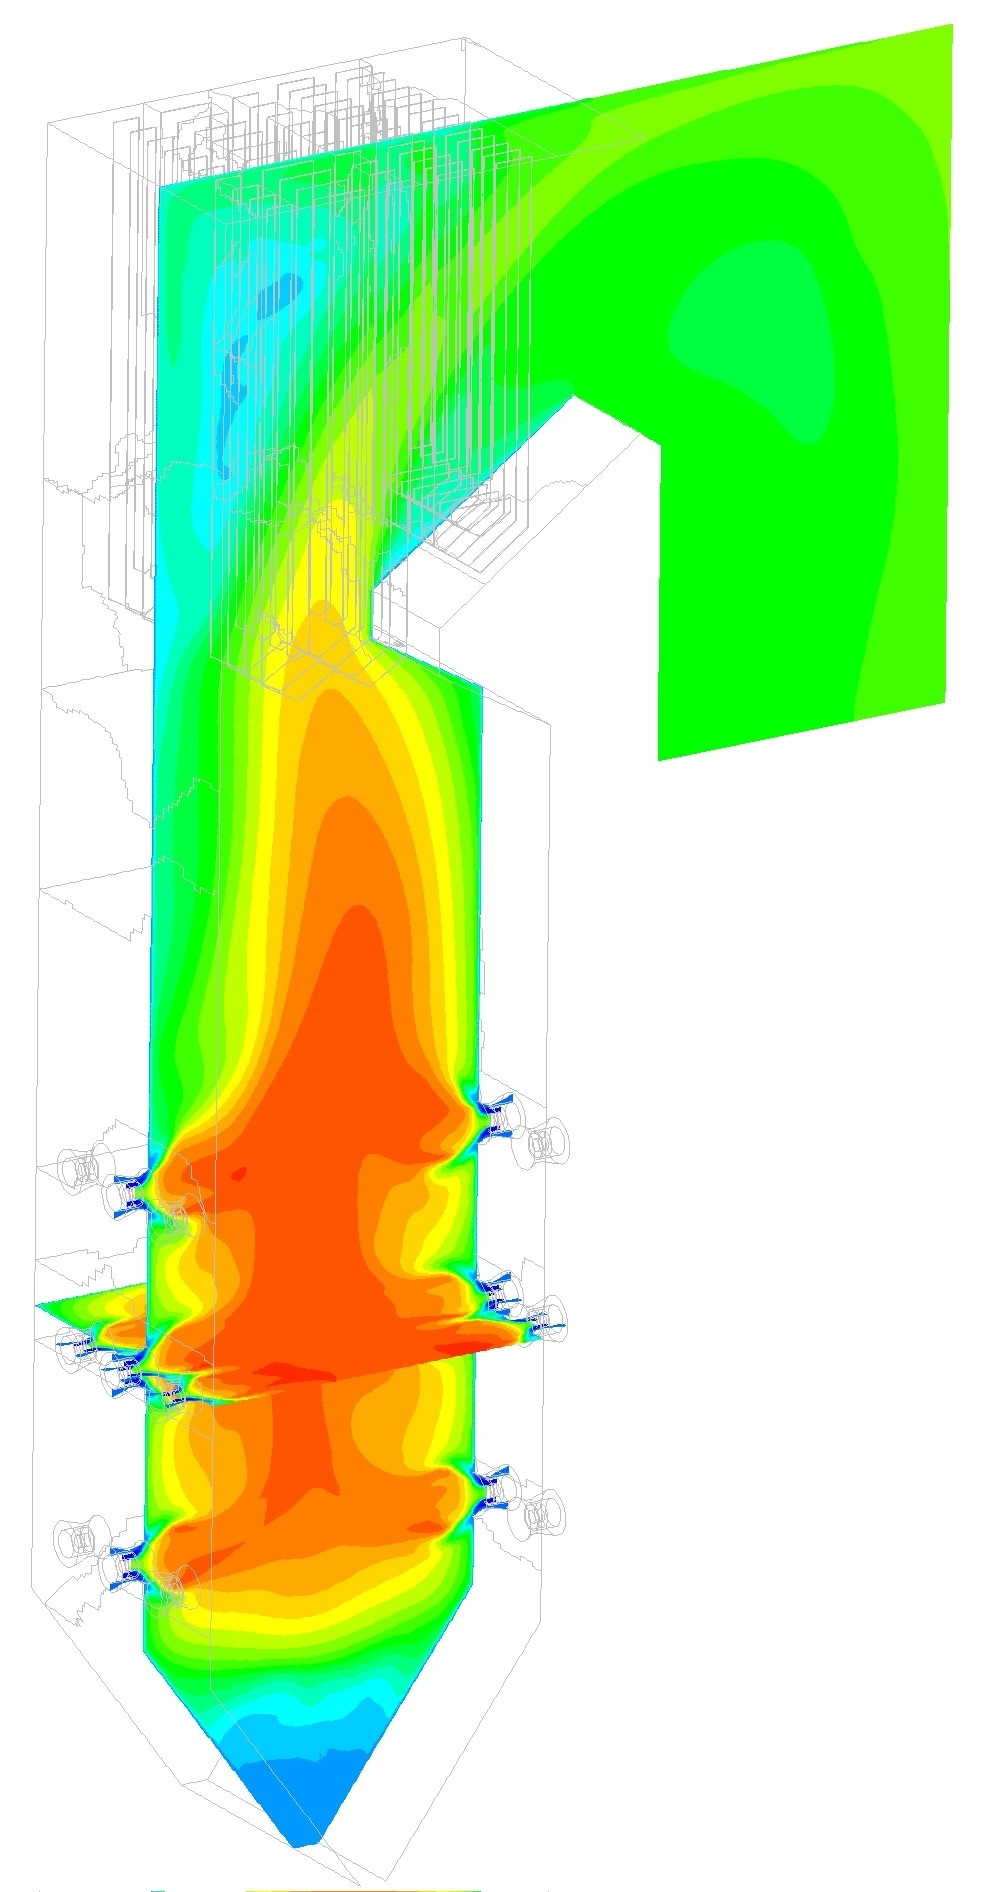
\includegraphics[scale = 0.0725]{60_temp}}\\
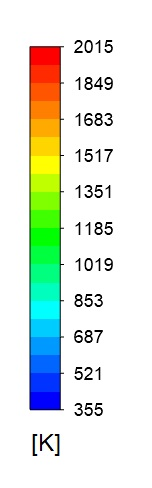
\includegraphics[scale = 0.3]{temp}
\subfloat[100\% case]{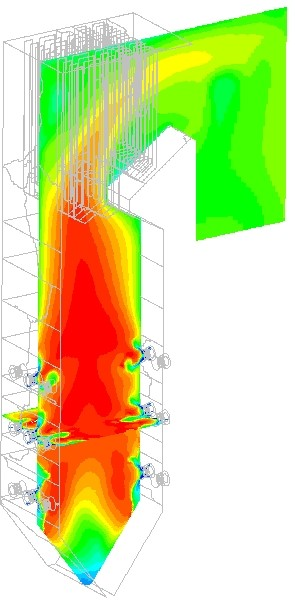
\includegraphics[scale = 0.224]{100_temp_spm}}
\hspace{10mm} 
\subfloat[81\% case]{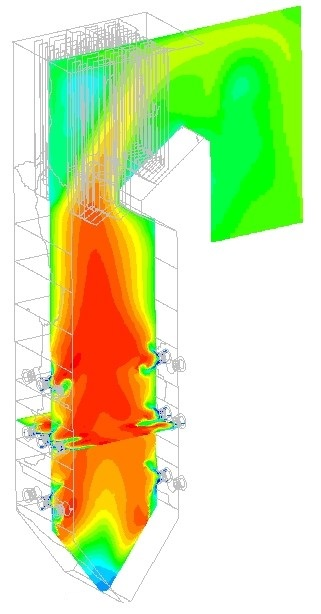
\includegraphics[scale = 0.224]{80_temp_spm}} 
\hspace{10mm} 
\subfloat[60\% case]{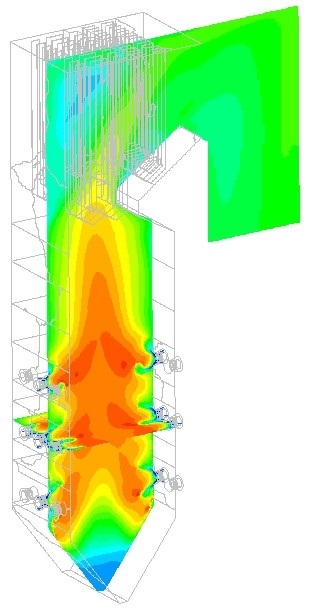
\includegraphics[scale = 0.224]{60_temp_spm}} 
\setlength{\belowcaptionskip}{0pt}
\caption{Temperature plots for the EL (a-c) and EE model (d-f) simulated load cases}
\label{fig_temp}
\end{figure}

The temperature contour plots of figure \ref{fig_temp} (d-f) illustrate the EE model's ability to sufficiently resolve the temperature field when compared to the EL model. The lower burners tend to initiate combustion closer to the burner leading to high temperatures. Due to the lack of velocity of the gas phase in this area, the high temperatures  are closer to the walls of the furnace leading to a higher heat flux observed as seen in figure \ref{fig_wall_heat} (d-f). In general the temperature and velocity fields are deemed sufficiently accurate for the purposes of surrogate model development, since the parameter of interest is the resolution of the wall flux field. The heat flux profiles are given in figure \ref{fig_wall_heat} (a-f). The EE model over predicts the wall fluxes in the lower half of the boiler, namely due to the high temperatures experienced in these zones in and around the bottom burners. The platen and HTSH radiant superheaters show similar flux profiles with the top half of the furnace illustrating sufficient agreement between the EL and EE models. The spatial distribution of the particles (expressed in $kg/m^3$) shown in figure \ref{fig_concentration} (a-f) highlights the EE model's ability to resolve the particle concentration throughout the domain for the various load cases. The general trend of the EE model is with sufficient accuracy when compared to the EL model.\\

\begin{figure}[h!]
\centering
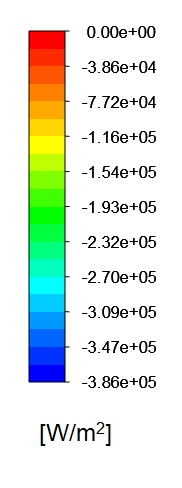
\includegraphics[scale = 0.3]{wall_heat}
\hspace{2mm}
\subfloat[100\% case]{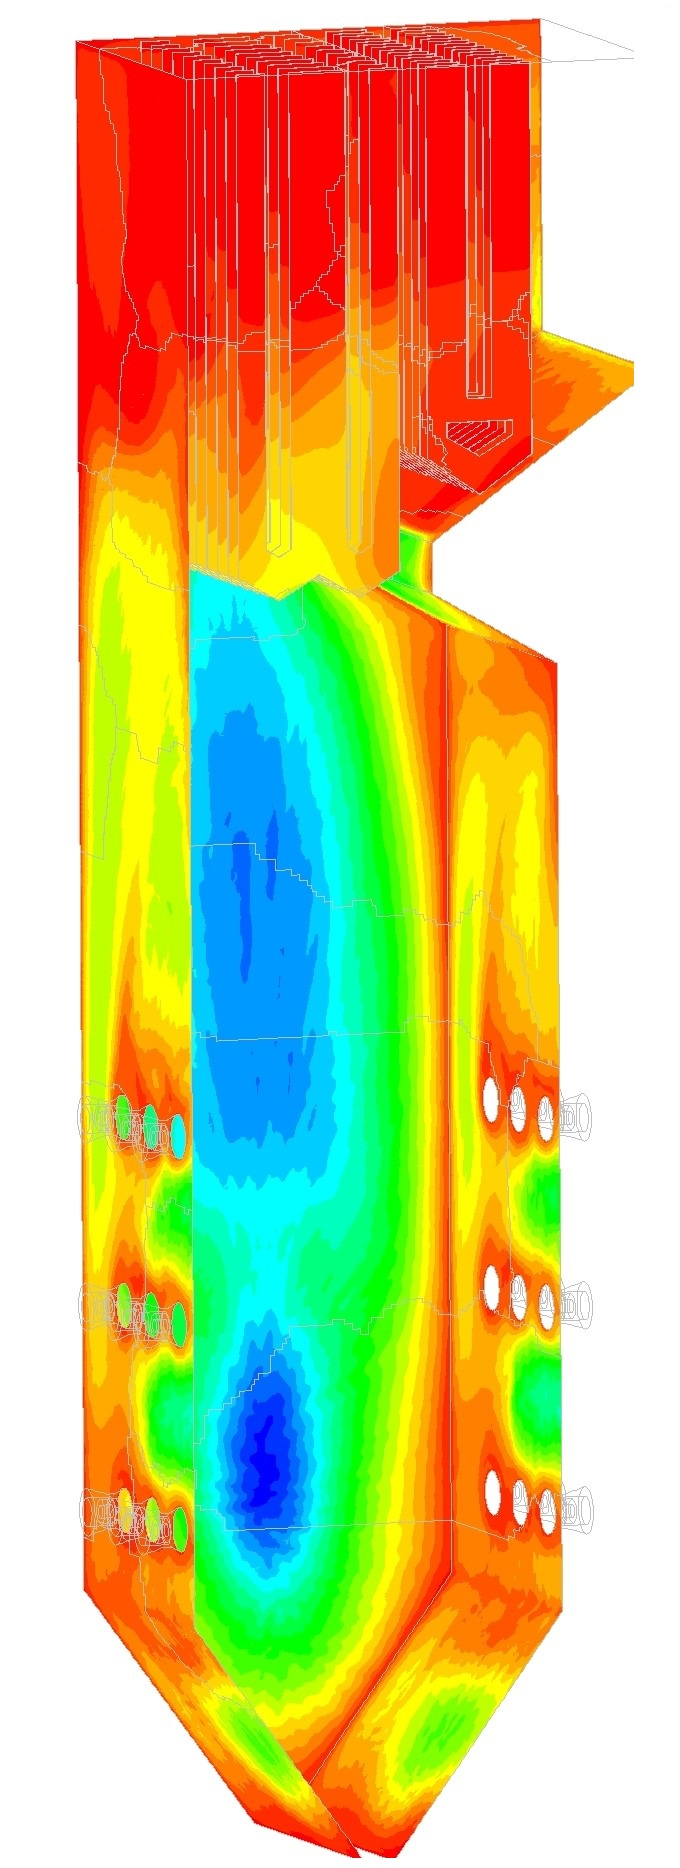
\includegraphics[scale = 0.075]{100_heat}} 
\hspace{10mm} 
\subfloat[81\% case]{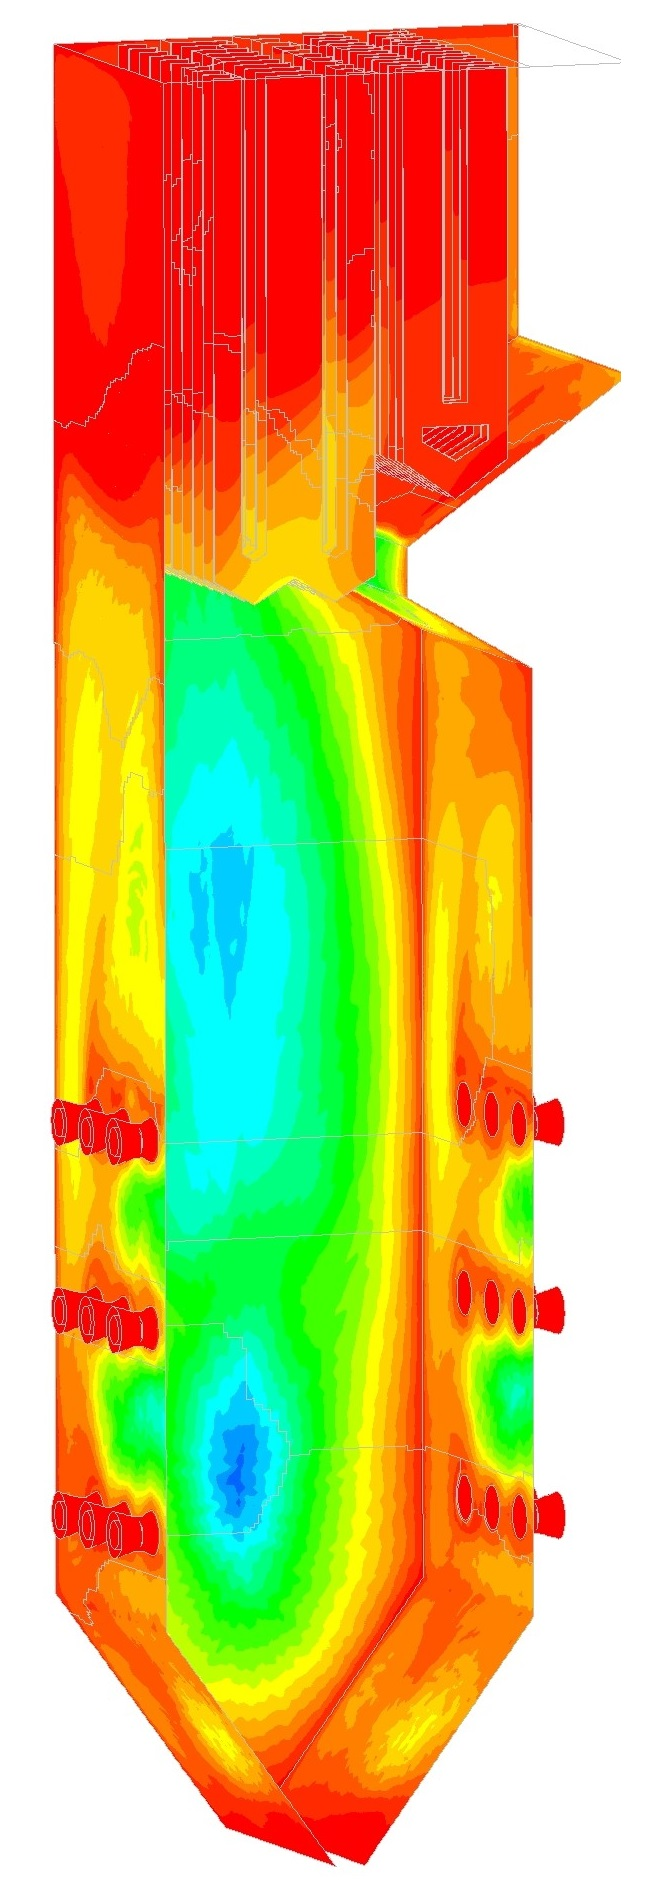
\includegraphics[scale = 0.075]{80_heat}}
\hspace{10mm} 
\subfloat[60\% case]{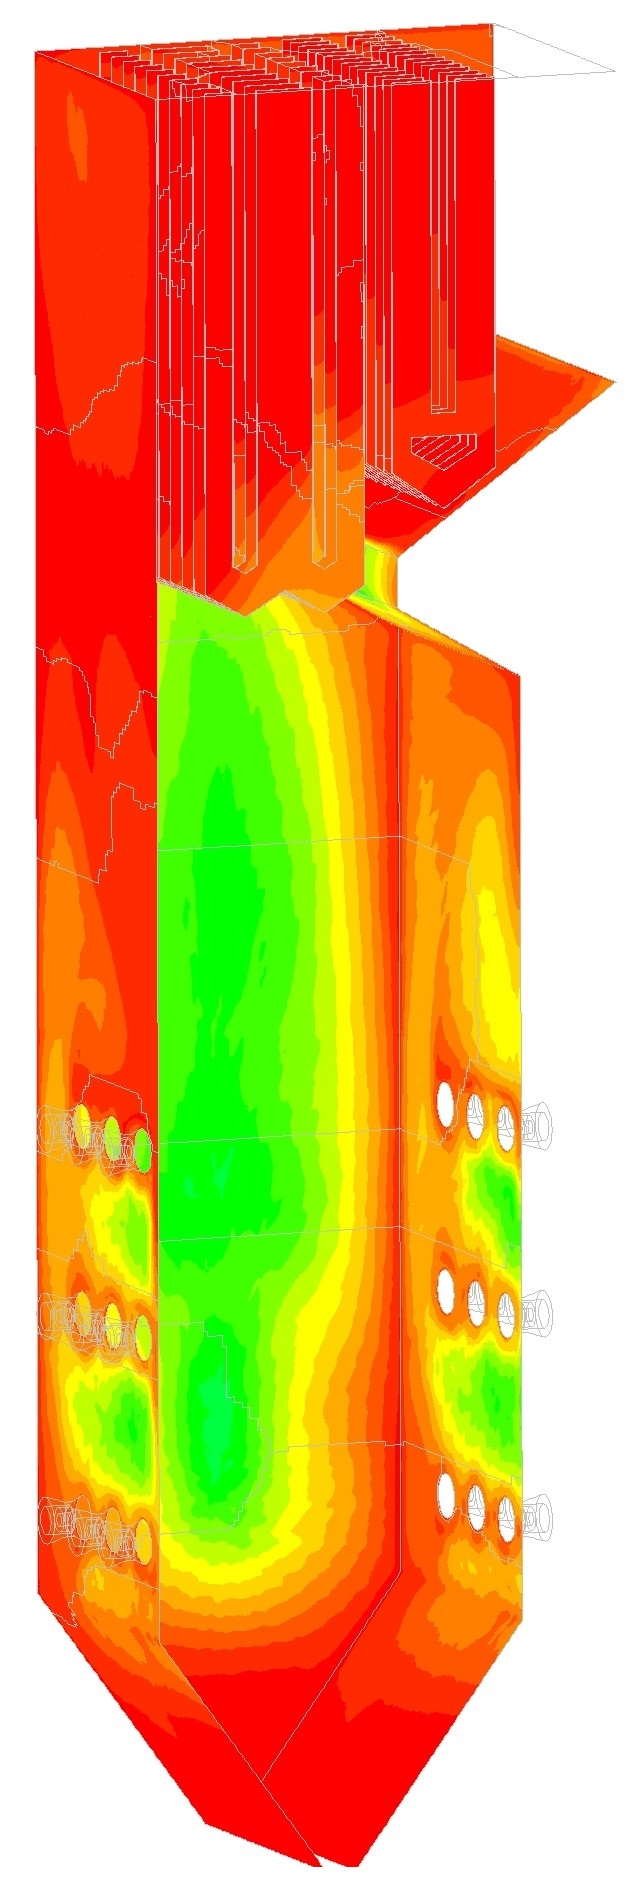
\includegraphics[scale = 0.075]{60_heat}}\\
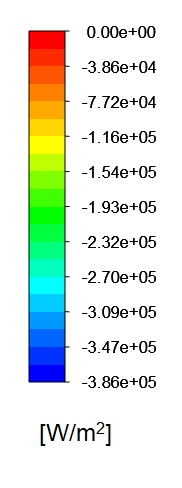
\includegraphics[scale = 0.3]{wall_heat}
\hspace{1mm}
\subfloat[100\% case]{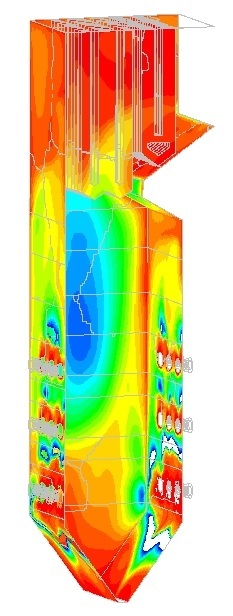
\includegraphics[scale = 0.225]{100_heat_spm}}
\hspace{9mm} 
\subfloat[81\% case]{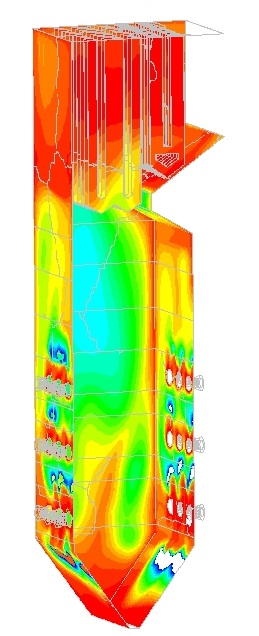
\includegraphics[scale = 0.22]{80_heat_spm}} 
\hspace{9mm} 
\subfloat[60\% case]{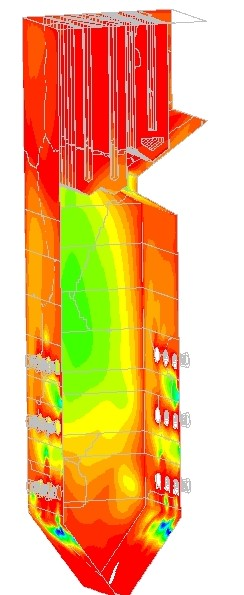
\includegraphics[scale = 0.225]{60_heat_spm}}
\setlength{\belowcaptionskip}{0pt} 
\caption{Wall heat flux profiles for the EL (a-c) and EE model (d-f) simulated load cases}
\label{fig_wall_heat}
\end{figure}

\begin{figure}[h!]
\centering
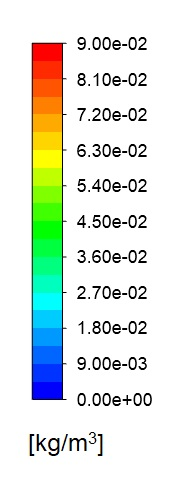
\includegraphics[scale = 0.25]{concentration}
\subfloat[100\% case]{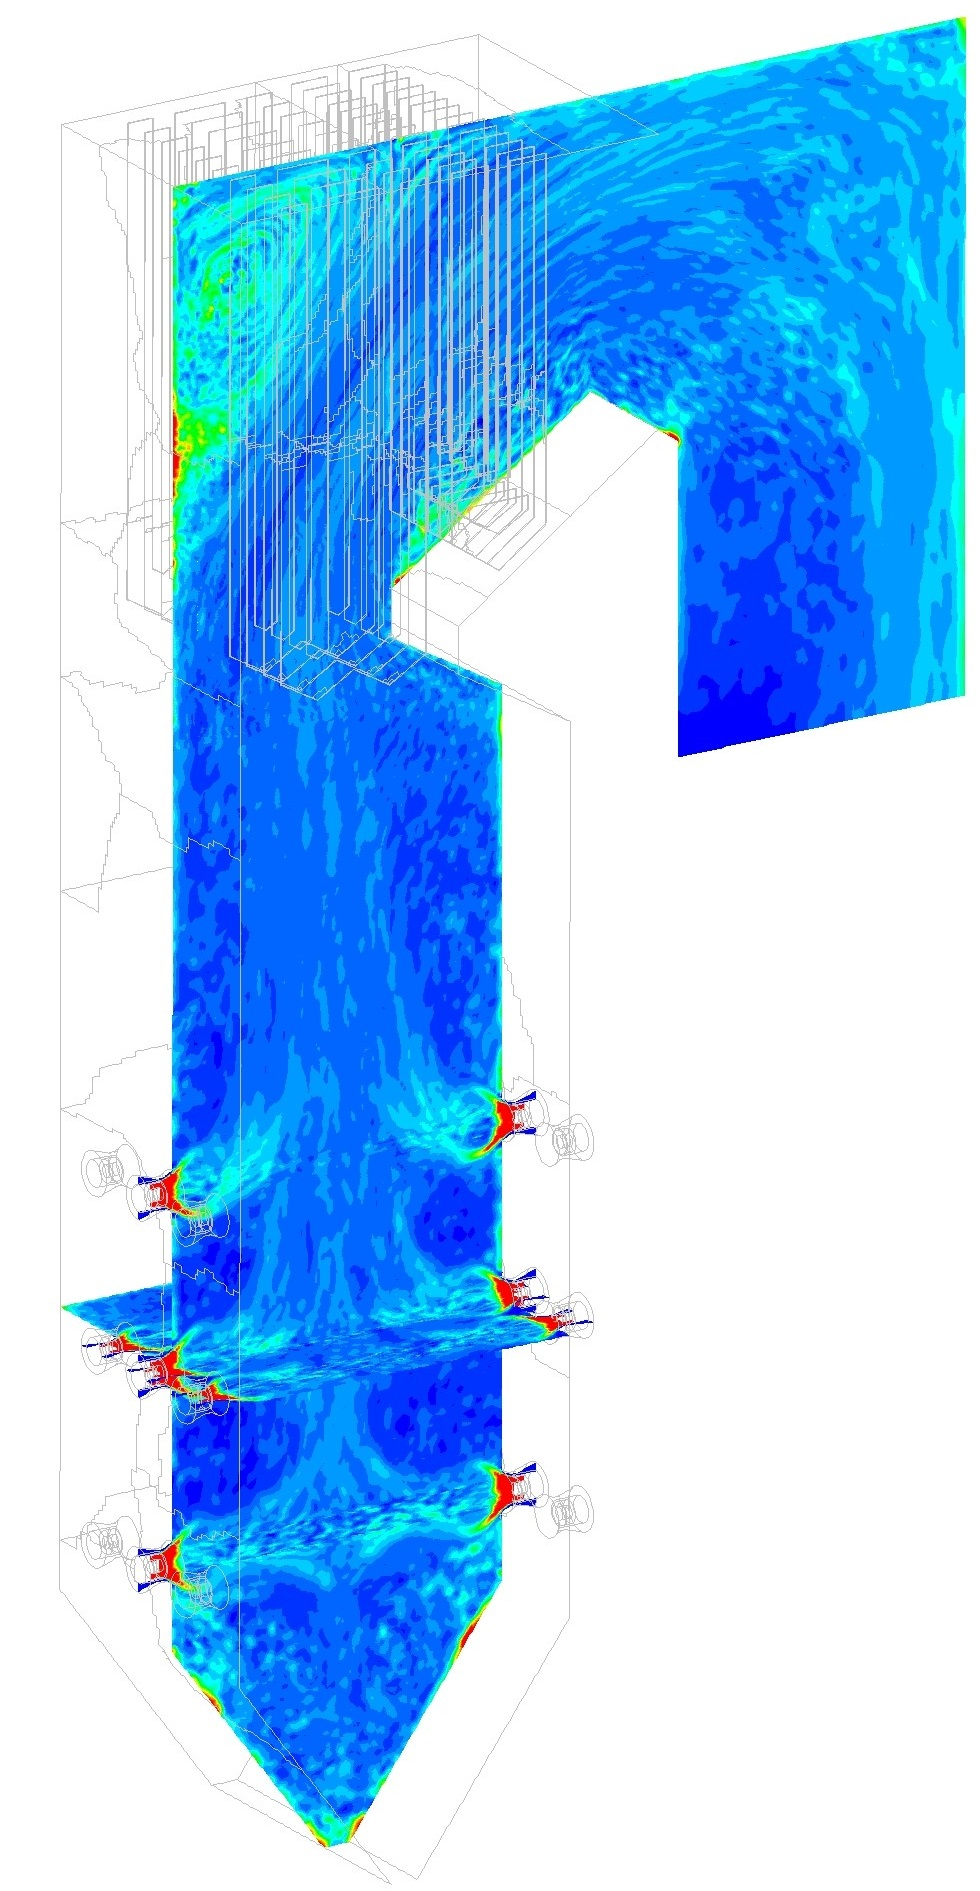
\includegraphics[scale = 0.065]{100_concentration}}
\hspace{10mm}  
\subfloat[81\% case]{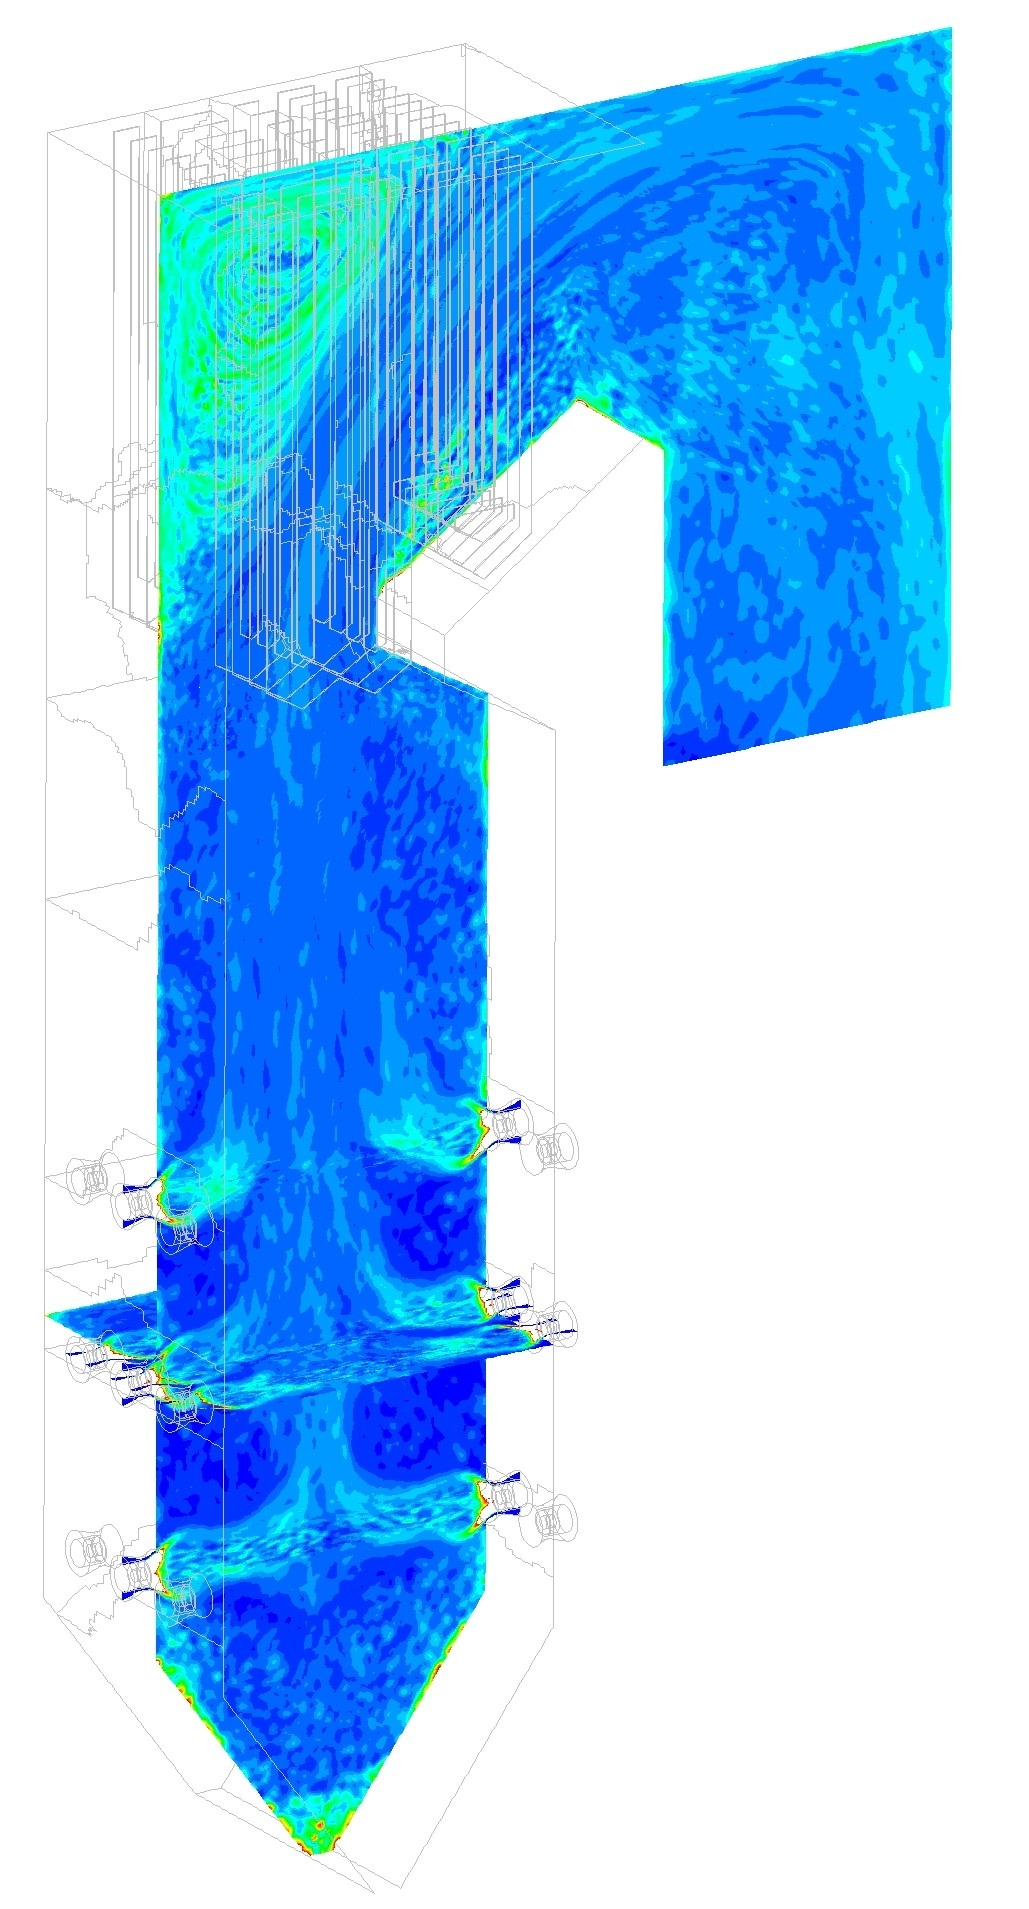
\includegraphics[scale = 0.065]{80_concentration}}
\hspace{10mm} 
\subfloat[60\% case]{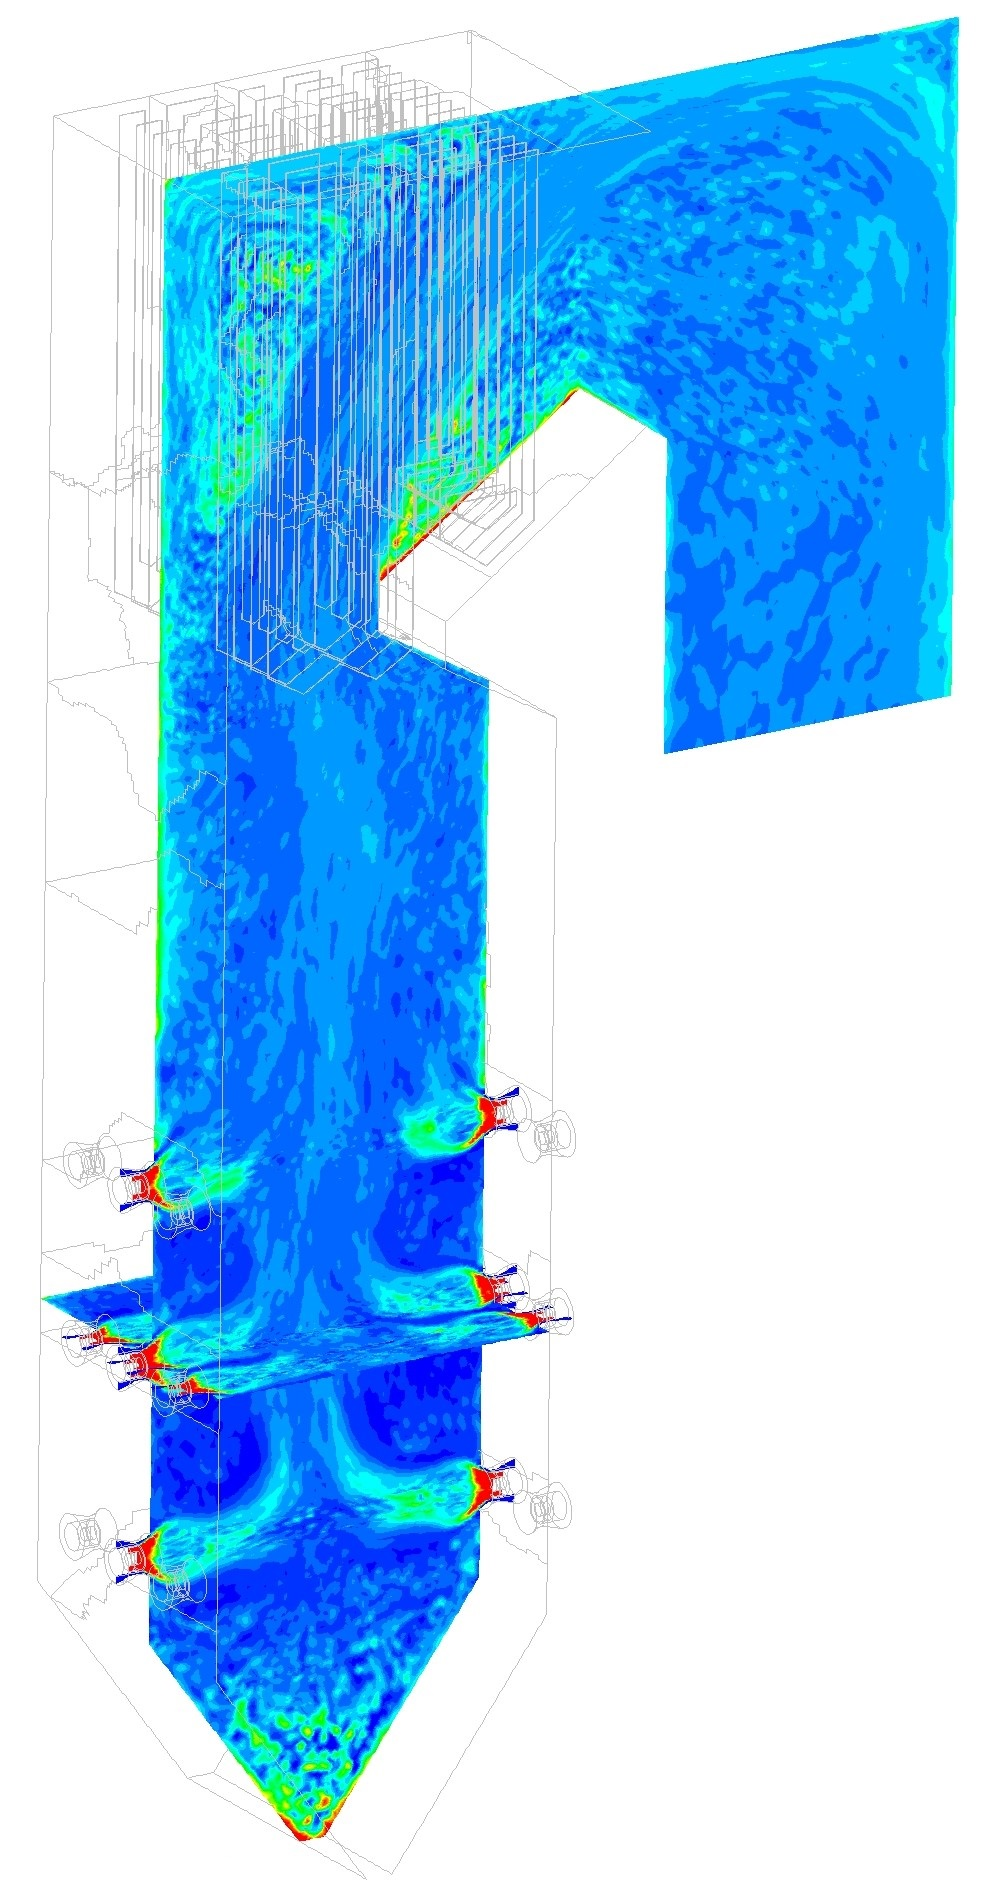
\includegraphics[scale = 0.065]{60_concentration}}\\
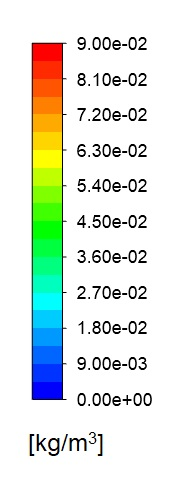
\includegraphics[scale = 0.25]{concentration}
\subfloat[100\% case]{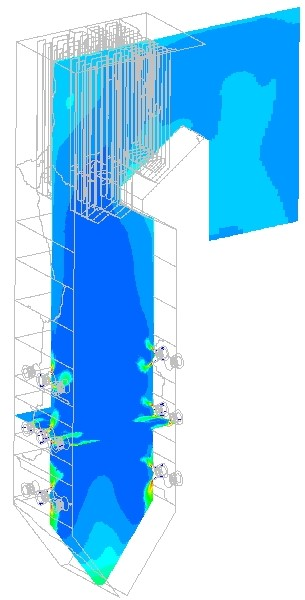
\includegraphics[scale = 0.2]{100_concentration_spm}}
\hspace{10mm} 
\subfloat[81\% case]{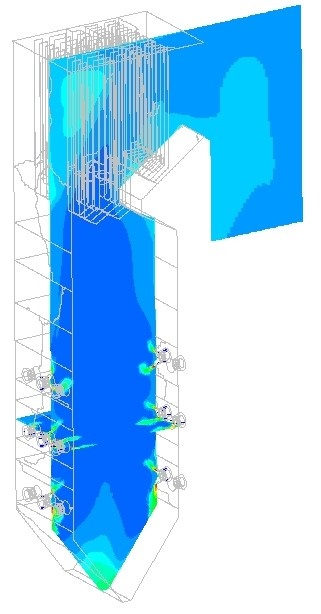
\includegraphics[scale = 0.2]{80_concentration_spm}}
\hspace{10mm}  
\subfloat[60\% case]{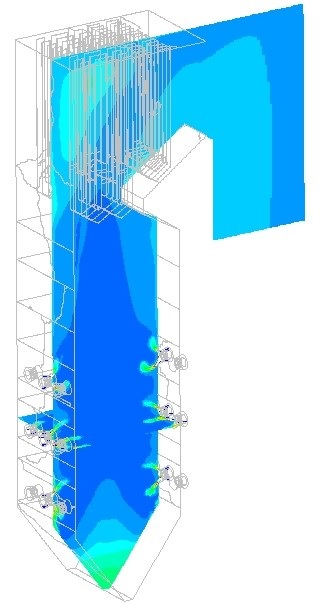
\includegraphics[scale = 0.2]{60_concentration_spm}}
\setlength{\belowcaptionskip}{0pt} 
\caption{Spatial particle concentration profiles for the EL (a-c) and EE model (d-f) simulated load cases}
\label{fig_concentration}
\end{figure}

\clearpage
\section{Conclusion}
The validation of a full scale 620 MWe boiler was conducted using a thermal non-equilibrium Eulerian-Eulerian model for three load cases, namely a 100\%, 81\% and 60\% steady-state loads. The validation cases include a comparison with results obtained by a numerical model using a Eulerian-Lagrangian approach and where applicable measured site data. The developed EE model demonstrated adequate performance in predicting the flow field, wall heat fluxes and fluid property distributions throughout the domain.The relative accuracy of the EE model ranged from 2 to 8\% for key parameters used in the study. The computational speedup, of 30\%, by using the EE model is a beneficial attribute when considering the EE models intended future use in the development of a CFD data-driven surrogate model. 

\section*{Acknowledgements}
The authors would like to thank the Eskom EPPEI program for funding this project and the Centre for High Performance Computing (CHPC, South Africa) for the computational resources provided for completing this work.

%
% BibTeX or Biber users please use (the style is already called in the class, ensure that the "woc.bst" style is in your local directory)
% \bibliography{name or your bibliography database}
%
% Non-BibTeX users please use
%

\begin{thebibliography}{}
%
% and use \bibitem to create references.
%

\bibitem{bohnstein}
M. von Bohnstein,  M. Richter, P. Schiemann, J. Str{\"{o}}hle, and B. Epple, Renewable and Sustainable Energy Reviews, \textbf{137}, (2021)

\bibitem{laubscher_1}
R. Laubscher, and P. Rousseau, Applied Thermal Engineering, \textbf{160}, (2019)

\bibitem{laubscher_2}
R. Laubscher, and P. Rousseau, International Journal of Heat and Mass Transfer, \textbf{137}, 506-522 (2019)

\bibitem{cai}
J. Cai, M. Handa, and  M.F. Modest, Combustion and Flame, \textbf{162}, 1550-1565 (2015)

\bibitem{wu}
Y. Wu, D. Liu, J. Ma, and X. Chen, Powder Technology, \textbf{342}, 48-61 (2018)

\bibitem{epple}
A.C. Benim,  B. Epple, and  B. Krohmer, Progress in Computational Fluid Dynamics, \textbf{5}, 345-361 (2005)

\bibitem{knaus}
H. Knaus, U. Schnell, and R.G. Klaus , Progress in Computational Fluid Dynamics , \textbf{1}, 194–207 (2001)

\bibitem{shih}
T.H. Shih, W.W. Liou, A. Shabbir, Z. Wang, and J. Zhu, Computers and fluids, \textbf{24}, (1995)


\bibitem{cengel}
Y.A. Cengel, and M.A. Boles, \textit{Thermodynamics: An engineering approach}, (McGraw Hill, Singapore, 2015)


\bibitem{gupta}
V..V. Ranade, and F.D. Gupta, \textit{Computational Modeling of Pulverized Coal Fired Boilers}, (CRC Press - Taylor {\&} Francis Group, Boca Raton, 2015) 101-105


\bibitem{sankar}
G. Sankar, D. Santhosh Kumar, and K.R. Balasubramanian, Fuel, \textbf{236}, 643-665 (2019)

\bibitem{sheng}
C. Sheng, B. Moghtaderi, R. Gupta, and T. F. Wall, Fuel, \textbf{83}, 1543-1552 (2004)

\bibitem{baum}
M.M. Baum, and P.J. Street, Combustion Science and Technology, \textbf{3}, 231-243 (1971) 


\bibitem{spalding}
D.B. Spalding, Symposium (International) on Combustion, \textbf{13}, (1970)

\bibitem{ansys}
\textit{ANSYS Fluent Theory Guide}, (Ansys Inc., 2021)

\bibitem{han}
A. Đugum and K. Hanjalić, Energy, (2018)

\bibitem{dibble}
V..V. Ranade, and F.D. Gupta, \textit{Combustion: Physical and chemical fundamentals, modelling and simulation, experiments, pollutant formation.}, (USA: Springer, 2006)


\bibitem{he}
B. He, Computational Fluids, \textbf{36}, 435-444 (2007)

\bibitem{smith}
T. Smith , Z. Shen , and J. Firedman, Journal of Heat Transfer, \textbf{104}, 602-608 (1982)

\bibitem{laubscher_3}
R. Laubscher,  and P. Rousseau, Energy, \textbf{195}, (2020)





% etc
\end{thebibliography}

\end{document}

% end of file template.tex

<div id='footer'><table width='100%'><tr><td class='right'><a href='http://fusioninventory.org/'><span class='copyright'>FusionInventory 9.1+1.0 | copyleft <img src='/glpi/plugins/fusioninventory/pics/copyleft.png'/>  2010-2016 by FusionInventory Team</span></a></td></tr></table></div>